\chapter{基于多维度特征的子痫前期识别模型的建立与分析}
\section{引言}
本章在上文构建的脉搏波新型时域波形描述特征集合与脉搏波原始采样点的基础上利用机器学习的相关算法完成了子痫前期识别模型的构建与分析工作。
本章首先对在上述过程中使用到的机器学习的典型算法的原理及评估模型优劣的性能指标进行了介绍。其次,基于新型时域波形描述特征集合与脉搏波原始采样点
分别完成了机器学习模型的筛选、模型超参数优化、特征贡献度分析与降维等研究工作。由于本研究使用的脉搏波数据规模较小,在进行机器模型构建过程中分别
按照原始波形与被试进行了数据划分。最后,对比了使用新型时域波形描述特征集合与脉搏波原始采样点分别得到的机器模型的结果的异同点,并分析了可能导致异同点的原因。

\section{机器学习算法原理与模型评价标准}
一般认为,机器学习是一门致力于研究通过计算的手段、利用已有的经验来改善系统自身性能的学科和艺术\cite{Zhou2016,Aurélien2018}。其中,Tom Mitchell对机器学习给出了一种最为经典的形式化定义:
计算机程序利用经验$E$学习任务$T$,其性能是$P$,如果针对任务$T$的性能$P$随着经验$E$不断增长,那么我们就说关于$T$与$P$,该程序对$E$进行了学习\cite{mitchell1997,Zhou2016}。
对计算机程序而言,$E$通常以数据的形式存在,因此机器学习也可以看成从相关数据中产生模型的算法过程,不显式编程是机器学习最典型的特征。
本文末附录D给出了部分机器学习领域常见的术语及其解释。

尽管机器学习的相关概念早在上世纪五十年代就已经被提出,但直到进入新世纪后,机器学习才真正迎来井喷式发展的黄金期。在过去二十年中,由于半导体电子计算机行业的充分发展,人类收集、传输、处理数据的能力取得了长足的进步,
人类各种社会活动中出现的海量数据具备了能够被挖掘、分析的硬件基础与需要被分析并加以利用的客观需求。在此背景下,机器学习受到了学者们的广泛关注并进入了蓬勃发展阶段,不论是理论基础方面亦或是应用研究方面都
得到了巨大的发展,取得了重大突破。目前,机器学习技术已经被成功应用在模式识别、数据挖掘、自然语言处理、语言识别、图像识别、芯片设计、信息检索及生物信息学等学科领域,
尤其是为交叉学科的发展研究提供了新的技术支撑与突破点\cite{Zhou2016,Aurélien2018,Li2017}。   

本小节将从本研究所使用到的机器学习的算法原理及评价使用机器算法训练得到的模型性能时的评价标准进行介绍。
\subsection{决策树与随机森林的算法原理}
监督学习是机器学习的重要研究方向,主要用于推断观察数据(也称为输入数据)与目标变量(因变量或标签)之间的潜在关系。
基于监督学习算法的经过良好训练的函数模型可以准确预测隐藏在不熟悉或未观察到的数据实例中的隐藏现象的类标签。
本研究的所使用的机器学习算法均属于此范畴。下面以决策树算法与随机森林算法为代表进行算法原理介绍。

一、决策树

决策树(Decision Tree,DT)是数据挖掘的经典算法之一,是一种类似流程图的树结构,可以用于连续数值型变量的回归预测及离散型数值型变量的分类问题\cite{Li2017,Liu2018}。
决策树算法的最显著优点是简单直观,易于可视化、可读性强。

1、决策树的结构与原理

分类决策树模型是对实例进行分类的树形结构的描述,如\autoref{fig:dt}所示。一般而言,决策树由结点和有向边组成,而结点又可分为内部结点与叶节点。其中,前者表示一个特征或属性,后者对应决策结果,一般是一个类\cite{Li2017,Zhou2016}。
决策树可以看成一个if-else规则的集合,决策树的根节点到叶节点的每条路径分别对应着一条规则:路径上的内部结点集合构成了规则的判断条件,而叶节点所属的具体类则对应着该规则的结论。
决策树的学习目的就是从训练数据集中集中归纳出一组分类规则,产生一颗与训练数据的矛盾小的、泛化能力强的逻辑判断树。
\begin{figure}[htbp]
      \centering
      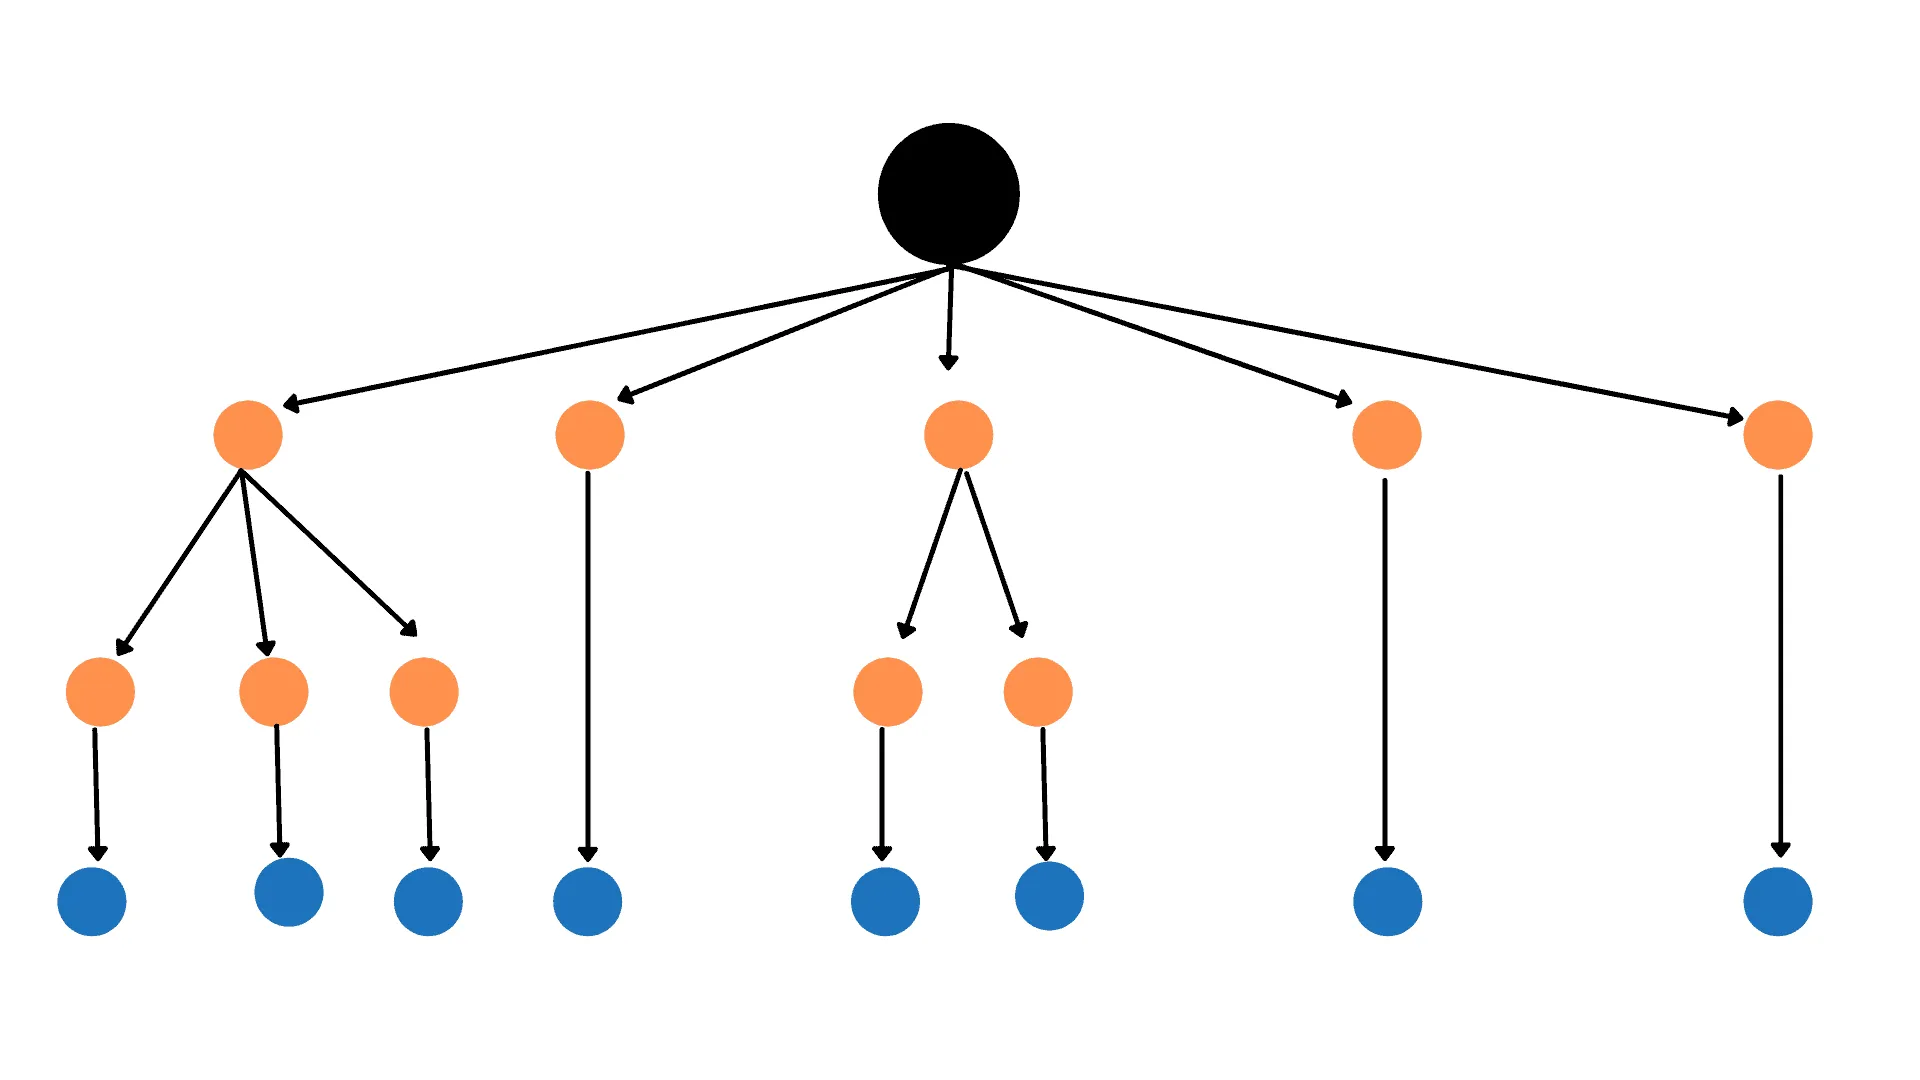
\includegraphics[width=.6\linewidth]{models/dt.png}
      \caption{\label{fig:dt}决策树模型示意}
\end{figure}

2、决策树的特征选择

为生成一颗分类能力强的决策树,一种可行的策略是只选取对分类效果有提升的特征参与构建。基尼指数(Gini index)与信息增益(information gain)是两种最常用的用于筛选最佳特征的指标。

基尼指数,也称为基尼不纯度,其定义为
\begin{equation}
      \label{equ:gini}
      G_i = 1 - \sum_{k=1}^n{p_{i,k}}^2
\end{equation}
其中,$p_{i,k}$是第$i$个节点上,类别为$k$的训练实例占比。基尼指数数值越大,样本集合的不确定性也越大。特别地,若样本集合$D$根据特征$A$是否取某一可能值$a$而被分割成$D_1$和$D_2$两部分,即
\begin{equation}
      \label{equ:daset}
      \left \{
      \begin{aligned}
            D_1 &= \{ (x,y) \in D \mid A(x) = a\} \\
            D_2 &= D - D_1
      \end{aligned}
      \right.
      \end{equation}
那么,在特征$A$的条件下,样本集合的基尼指数可以表示为
\begin{equation}
      \label{equ:ginia}
      G(D,A) = \frac{|D_1|}{|D|}G(D_1) + \frac{|D_2|}{|D|}G(D_2)
\end{equation}
其中,$|D|$表示样本集合$D$的样本数量。\autoref{equ:ginia}描述了$D$经特征$A=a$分割后的不确定性,此时,筛选最佳特征的过程可以转换为寻找使\autoref{equ:ginia}取值最小的特征$A$的具体数值。

另一方面,信息增益是在引入了信息论中的信息熵(information entropy)概念进行定义的并计算使用的,其作用与具体使用方法与基尼指数类似,这里不再进行赘述\cite{Zhou2016,Li2017}。

3、决策树的生成

决策树的生成构建过程就是递归地选择最优特征,并根据最优特征对训练数据进行分割,使该分割对各个新的子数据集有最优分类效果的过程。其中,最经典生成算法包括ID3(Iterative Dichotomiser 3,第三代迭代二分器)决策树学习算法、
C4.5(Classifier 4.5,第4.5代分类器)决策树学习算法及CART(classification and regression tree,分类与回归树)决策树学习算法等三种\cite{quinlan1986,quinlan1993,breiman1984}。
在这三种算法中,只有CART算法生成的决策树既可以执行分类任务也可以执行回归任务,故CART算法的应用也最为广泛。

CART算法采用最小基尼指数来选择特征,生成的决策树为二叉树。其工作的基本原理如\autoref{alg:cart}所示。
\begin{breakablealgorithm}
      \caption[CART生成算法]{CART递归生成算法\cite{Li2017}}
      \label{alg:cart}
      \begin{algorithmic}[1] %每行显示行号
            \Require 训练数据集$D$。
            \Ensure CART决策树。
            \State 建立一颗空树$CART$,设该树的根结点为$root$。
            \Function{GenerateCart}{$CART,D_c,root$}
                  \State $D_c$为当前结点的训练数据集,计算现有特征对该数据集的基尼指数。对每一个特征$A$,对其可能取的每个值$a$,根据样本点对$A=a$的测试为“是”或“否”将$D_c$分割成$D_l$与$D_r$两部分,使用\autoref{equ:ginia}计算$A=a$时的基尼指数。
                  \State 在所有可能的特征$A$以及它们所有可能的切分点$a$中,选择基尼指数最小的特征及其对应的切分点作为最有特征与最优切分点。
                  \State 依最优特征与最优切分点,从现结点生成两个子节点$left$与$right$,将训练数据集依特征分配到两个子节点中去,即$D_l$与$D_r$。更新当前$CART$。
                  \If {结点中的样本个数小于预定阈值 \textbf{or} 样本集的基尼指数小于预定阈值 \textbf{or} 没有更多特征}
                  \State \Return{$CART$}
                  \Else    
                  \State \Call{GenerateCart}{$CART,D_l,left$}
                  \State \Call{GenerateCart}{$CART,D_r,right$}
                  \EndIf
            \EndFunction
      \end{algorithmic}
\end{breakablealgorithm}

4、决策树的剪枝

为防止决策树出现过拟合的情况,通常都会对过于“茂密”的树进行剪枝(pruning)处理。决策树的剪枝方法可以分为预剪枝与后剪枝两大类。
前者的工作原理是在决策树的生长阶段就对其进行一定的限制,包括限制树最大生长深度、限制决策树生成的最多叶节点数量等。
后剪枝则是在决策树得到完全生长之后进行,其处理算法也更复杂、训练时间等开销也更大\cite{Zhou2016,Liu2018}。

二、随机森林

随机森林是一种在Bagging算法基础上发展起来的集成学习算法,最早由Leo Breiman于2001年提出\cite{breiman2001}。

1、Bagging

为获得泛化性能强的不同的基学习器,一种可行的策略是对所有学习器使用同一种训练算法,但是在训练集的不同随机子集上进行训练,使这些基学习器的能够有一定的差异。
\autoref{fig:bp}所示,在上述过程的随机子集的建立过程中,若对原始数据样本的采样后放回,这种方法即为bagging;与之对应的,采样后不放回的方法称为pasting\cite{Aurélien2018,Zhou2016}。
由于bagging方法可以获得的随机子集数量要远远高于pasting方法,bagging方法应用得也更加广泛。
\begin{figure}[htbp]
      \centering
      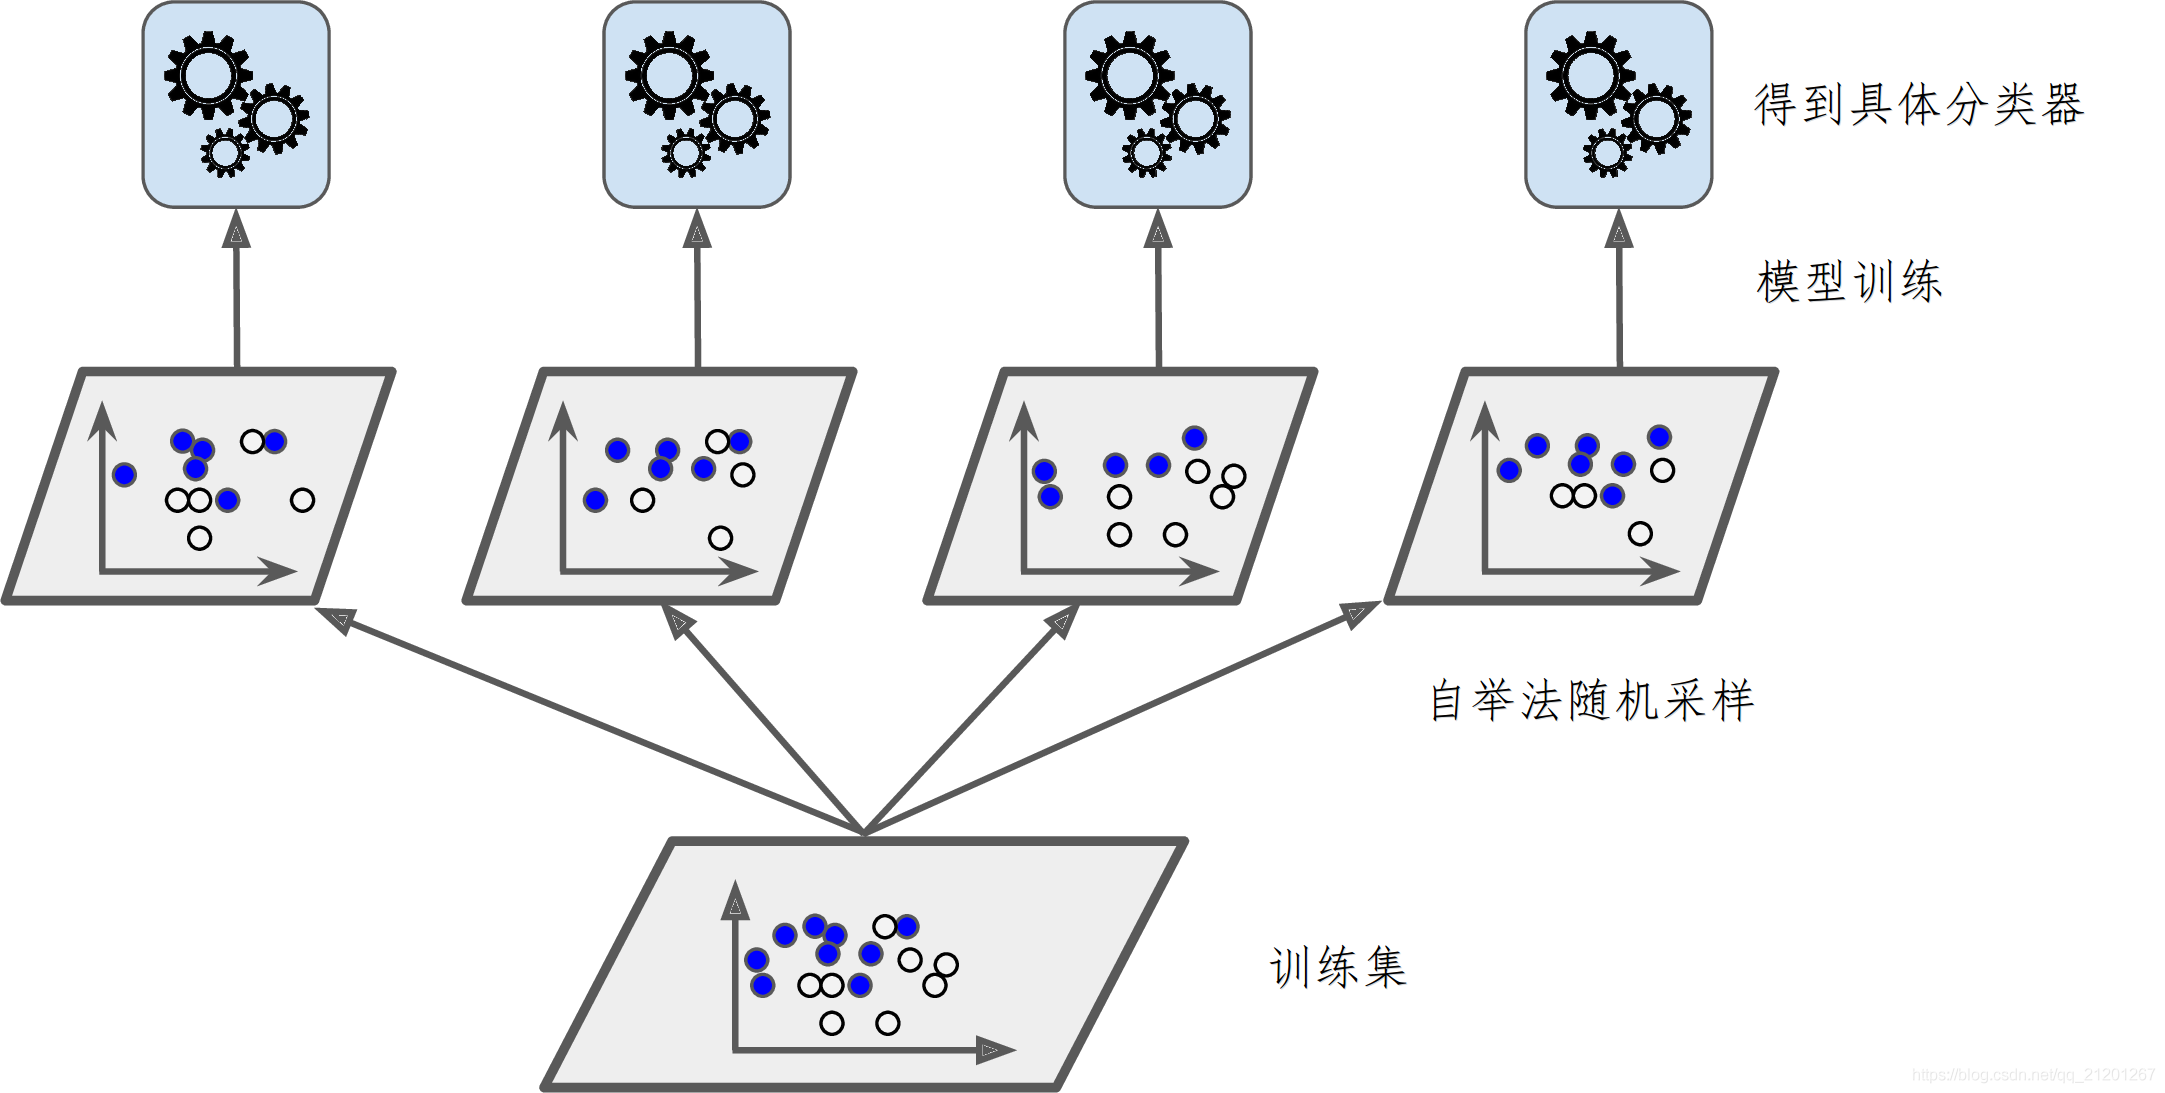
\includegraphics[width=.6\linewidth]{models/bp}
      \caption[Bagging与Pasting示意]{\label{fig:bp}Bagging与Pasting示意\cite{Aurélien2018}}
\end{figure}

当使用有采样后即放回的方法从包含$m$个原始样本的训练集$D$抽取出$m$个新的样本构成此次训练数据集$D_{bs}$时,显然,$D$有部分数据样本在$D_{bs}$重复出现,部分数据则从未被抽样过。
易知样本在$m$次均未被抽中的概率为$(1-\frac{1}{m})^m$,当$m \to \infty$时,
\begin{equation}
      \label{equ:me}
      \lim_{m \to \infty}{(1-\frac{1}{m})}^m = \frac{1}{e} \approx 0.368
\end{equation}
\autoref{equ:me}说明约有36.8\%的原始样本未出现在采样集$D_{bs}$中,这部分数据可以作为当前训练算法的测试集。

按上述思想,可从原始样本训练集$D$采样得到$T$个包含$m$个训练样本的采样集,基于这些采样集,使用特定的机器学习算法可以训练得到$T$个基学习器,结合这些基学习器的输出即为Bagging算法
的基本流程,如\autoref{alg:bagging}所示。投票法和平均法是Bagging在进行基学习器的输出时常采用的策略。
\begin{breakablealgorithm}
      \caption[Bagging算法]{Bagging算法\cite{Zhou2016}}
      \label{alg:bagging}
      \begin{algorithmic}[1] %每行显示行号
            \Require 训练集$D=\{(x_1,y_1),(x_2,y_2),\dots,(x_m,y_m)\}$;基学习算法$\xi$;训练轮数$T$。
            \Ensure $H(x)=\arg \max \limits_{y \in Y} \sum_{t=1}^T \mathbb{I}(h_t(x)=y)$,其中$\mathbb{I}(.)$为指示函数,在$.$为真或假时函数值分别为1或0。
            \For {$t=1,2,\dots,T$}
                  \State 从原始训练集$D$自助采样得到此次的样本分布$D_{bs}$
                  \State $h_t=\xi (D,D_{bs})$
            \EndFor
      \end{algorithmic}
\end{breakablealgorithm}

2、随机森林

如\autoref{fig:rf}所示,随机森林算法是由多棵\autoref{fig:dt}所示的决策树构成,这些决策树一般都是经过充分生长的、未经剪枝处理的CART决策树。
而“随机”一词有两重含义,首先是同Bagging算法一样,每棵决策树在训练时使用的训练样本是随机抽取的;其次,与\autoref{alg:cart}所示的一般CART决策树生成算法不同,随机森林中的CART
决策树在生长时并不是在当前结点的$d$个属性集合$A$中选取最优特征及其最优切分点,而是先从$A$中随机生成一个包含$k$个属性子集的$A_{bs}$,随后再从$A_{bs}$中选择最优属性进行划分\cite{Zhou2016,Liu2018,breiman2001}。其中,$k$的推荐取值为
$\lfloor \log_2m + 1 \rfloor$\cite{breiman2001}。

\begin{figure}[htbp]
      \centering
      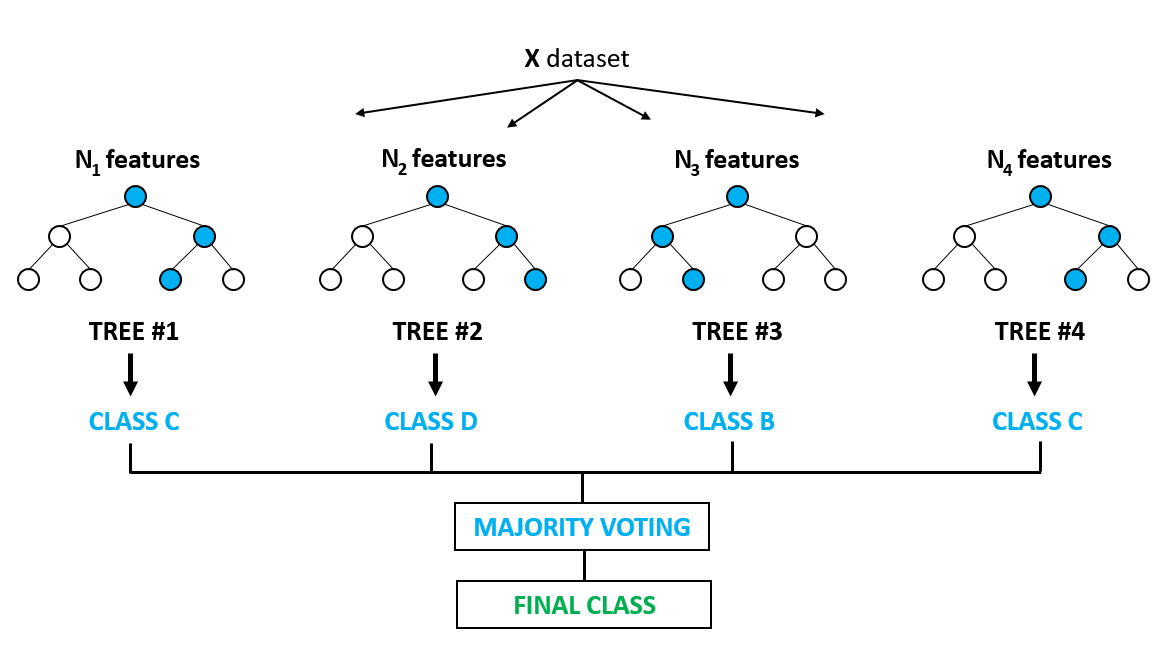
\includegraphics[width=.6\linewidth]{models/rf}
      \caption{\label{fig:rf}随机森林示意}
\end{figure}

对回归问题而言,随机森林算法的输出是所有决策树的输出的均值;而对分类任务而言,算法输出是所有决策树输出投票的结果。随机森林在树的生长过程中的两次随机使决策树具有更大的多样性,相当于用更高的偏差换取更低的方差。因此,
最终的集成结果有着出色的泛化性能,有效避免了单决策树可能导致的过拟合问题。随机森林算法运行速度快、准确率高且泛化性能优秀,被誉为“代表集成学习技术水平的方法”\cite{Zhou2016,Liu2018}。

此外,随机森林算法往往也会在特征选择的过程中得到应用\cite{Aurélien2018}。重新考察\autoref{fig:dt}中的决策树可以发现,越靠近根结点位置的特征对决策过程的重要程度也越高,而不重要的特征多出现在靠近结点的位置、甚至不出现在决策树中。
因此,特征的重要性(或贡献度)可以通过计算其在随机森林众多决策树的平均深度来进行量化衡量。

\subsection{机器学习模型的评价标准}
为量化描述机器学习算法训练得到的模型的性能表现,学者们提出了多种衡量指标。

一、混淆矩阵及其衍生指标

混淆矩阵(confusion matrix)是评估分类器分类效果优劣的常用工具\cite{Zhou2016,Aurélien2018}。其总体思路就是分别统计A类别实例被划分成B类别实例的数目。理论上混淆矩阵的行列没有上限,而在实际应用中,二分类任务的混淆矩阵是最常见的。
此时,将样例依据其真实所属类别与分类器预测类别进行组合可得到四种结果:真阳性(true positive,TP)、假阳性(false positive,FP)、真阴性(true negative,TN)及假阴性(false negative,TN),如\autoref{tab:cm}所示。此时显然有
$TP+FP+TN+FN=\text{样例总数}$。
\begin{table}[htbp]
      \centering
      \caption{\label{tab:cm}二分类任务的混淆矩阵}
      \begin{tabular}{ccc}
      \toprule
      \multicolumn{1}{c}{\multirow{2}[4]{*}{\textbf{真实情况}}} & \multicolumn{2}{c}{\textbf{预测结果}} \\
            \cmidrule{2-3}          & 阳性(1) & 阴性(0) \\
      \midrule
      阳性(1) & 真阳性(TP) & 假阴性(FN) \\
      阴性(0) & 假阳性(FP) & 真阴性(TN) \\
      \bottomrule
      \end{tabular}%
\end{table}%

为量化分类器的具体性能,人们在混淆矩阵的基础上衍生定义了一系列数字指标,包括查全率(recall)、查准率(precison)、准确率(accuracy)及特异性(specificity)等,如\autoref{equ:measures}所示。
\begin{equation}
      \label{equ:measures}
      \left \{
      \begin{aligned}
            Recall      &=\frac{TP}{TP+FN}         \\
            Precison    &=\frac{TP}{TP+FP}          \\
            Accuracy    &=\frac{TP+TN}{TP+FP+TN+FN} \\
            Specificity &=\frac{TN}{TN+FP}       \\
      \end{aligned}
      \right.
\end{equation}
其中,查全率亦称召回率、灵敏性(sensitivity)或真阳性率(true positive rate,TPR),查准率亦称精准率,特异性亦称真阴性率。查全率与查准率是应用的最广泛的两个指标\cite{Zhou2016,Aurélien2018}。
一般而言,查全率与查准率是对相互矛盾的度量指标,一个指标性能的提高意味着另一个指标性能的下降。通常只有在简单分类任务中,
才能同时获得较高的查准率与查全率。这称为精度-召回率权衡。为评估查全率与查准率均不相等的分类器性能,人们进一步定义了$F_1\text{分数}$,如\autoref{equ:f1}所示。
\begin{equation}
      \label{equ:f1}
      F_1=\frac{2}{\frac{1}{Precison}+\frac{1}{Recall}}=\frac{2\cdot Precison\cdot Recall}{Precison+Recall}=\frac{TP}{TP+\frac{FN+FP}{2}}
\end{equation}
$F_1\text{分数}$是召回率与精准率的谐波均值。召回率与精准率相近的分类器易获得更高的$F_1\text{分数}$。

在评估分类器性能时需要根据场景,从\autoref{equ:measures}与\autoref{equ:f1}中灵活选取恰当的评价指标。

二、ROC曲线、AUC与约登指数

受试者工作特征(Receiver Operating Characteristic,ROC)曲线是另一种常用于二分类问题的分析工具。ROC绘制的是真阳性率和假阳性率(false positive rate,FPR)之间的变化关系,其中
\begin{equation}
      \label{equ:fpr}
      FPR=\frac{TN}{TN+FP}=1-Specificity
\end{equation}
因此,ROC曲线也被称为灵敏度与1-特异性曲线。绘制曲线时,以分类器的预测结果对样例进行升序排列,依次将样本作为阳性进行预测,计算对应的TPR与FPR后,可得一坐标点$({FPR}_i,{TPR}_i)$,最后将所有坐标点连线即可,如\autoref{fig:roc}所示。
其中,虚线表示纯随机分类器的ROC曲线,理想性能的分类器应无限逼近左上角,即坐标点$(0,1)$。
\begin{figure}[htbp]
      \centering
      \includegraphics[width=.6\linewidth]{data_plan/roc}
      \caption[ROC曲线与AUC数值]{\label{fig:roc}ROC曲线与AUC数值。各分类器的AUC具体数值参见图例。}
\end{figure}

在衡量多个分类器性能优劣时,常将分类器对应的ROC曲线下面积作为判据,即为AUC(Area Under Curve)。纯随机分类器ROC的AUC数值为0.5,而理想分类器ROC的AUC数值为1,如\autoref{fig:roc}所示。

此外,约登指数(Youden Index)也是用来评价分类器效果的一个指标。若在评估分类器性能时,给予将分类器假阴性和假阳性以相同权重,即可应用约登指数
\begin{equation}
      \label{equ:yi}
      \begin{aligned}
            YI&=Sensitivity-(1-Specificity)\\
            &=Sensitivity+Specificity-1
      \end{aligned}
\end{equation}
一般认为,当YI取值最大时,此时对应的分类阈值为最佳阈值\cite{cwl}。

\section{基于新型时域波形描述特征集合生成的模型及分析}

\subsection{按照全部波形抽样}
一、算法初筛

在按照全部波形进行抽样的数据集的基础上,为检验新型时域波形描述特征集合中各指标表征子痫前期的能力,本研究使用了监督学习的多种算法进行了子痫前期识别模型的试探性研究\cite{scikit-learn}。
此过程共使用了随机梯度下降、决策树、K近邻、高斯朴素贝叶斯、逻辑回归、线性支持向量机、核支持向量机、C-支持向量机及多层感知机等9种基本分类算法。在使用上述算法构建模型时,各算法的超参数均未经调整,使用了默认数值设置\cite{scikit-learn}。
通过这9种算法构建的模型(以下简称为模型)在训练集与测试集上的结果如\autoref{tab:model_screen}所示,其中训练集相关数据是对原始训练集数据经过5层交叉验证后得到的。
\begin{landscape}
      \zihao{-5}
      \begin{longtable}{m{3cm}<{\centering}m{1.7cm}<{\centering}m{2.3cm}<{\centering}m{1cm}<{\centering}m{1cm}<{\centering}m{1cm}<{\centering}m{1cm}<{\centering}m{1cm}<{\centering}m{2cm}<{\centering}m{1cm}<{\centering}m{1cm}<{\centering}m{1cm}<{\centering}m{1cm}<{\centering}}
            \caption{初筛结果}\\
            \label{tab:model_screen}\\
            \toprule
            &  & \multicolumn{6}{c}{\textbf{训练集(5层交叉验证)}} & \multicolumn{5}{c}{\textbf{验证集}}                                                                                                                                                                                                      \\
            \multirow{-2}{*}{\textbf{模型类型}} & \multirow{-2}{*}{\textbf{训练时间}} & \textbf{混淆矩阵} &  \textbf{精确率} &  \textbf{召回率} &  \textbf{F1值} &  \textbf{准确率} &  \textbf{AUC} &  \textbf{混淆矩阵} &  \textbf{精确率} &  \textbf{召回率} &  \textbf{F1值} &  \textbf{准确率}    \\
            \midrule
            \endfirsthead
            \caption[]{(续)}\\
            \midrule
            &  & \multicolumn{6}{c}{\textbf{训练集(5层交叉验证)}} & \multicolumn{5}{c}{\textbf{验证集}}                                                                                                                                                                                                      \\
            \multirow{-2}{*}{\textbf{模型类型}} & \multirow{-2}{*}{\textbf{训练时间}} & \textbf{混淆矩阵} &  \textbf{精确率} &  \textbf{召回率} &  \textbf{F1值} &  \textbf{准确率} &  \textbf{AUC} &  \textbf{混淆矩阵} &  \textbf{精确率} &  \textbf{召回率} &  \textbf{F1值} &  \textbf{准确率}    \\
            \midrule
            \endhead 
            \midrule
            \endfoot
            \bottomrule
            \endlastfoot
            随机梯度下降      &   6.17 s  &     $\left[ \begin{array}{cc} 2165 & 380 \\ 1164 & 2582 \end{array} \right]$ & 87.2\% & 68.9\% & 77.0\% & 75.5\% & 0.876 &
            $\left[ \begin{array}{cc} 328 & 308 \\ 22 & 915 \end{array} \right]$ & 74.8\% & 97.7\% & 84.7\% & 79.0\% \\
            决策树            &   5.24 s  &     $\left[ \begin{array}{cc} 2241 & 304 \\ 635 & 3111 \end{array} \right]$ & 91.1\% & 83.0\% & 86.9\% & 85.1\% & 0.907 &
            $\left[ \begin{array}{cc} 584 & 52 \\ 174 & 763 \end{array} \right]$ & 93.6\% & 81.4\% & 87.1\% & 85.6\% \\
            K近邻算法      &   3.08 s  &     $\left[ \begin{array}{cc} 2347 & 198 \\ 237 & 3509 \end{array} \right]$ & 94.7\% & 93.7\% & 94.2\% & 93.1\% & 0.974 &
            $\left[ \begin{array}{cc} 594 & 42 \\ 63 & 874 \end{array} \right]$ & 95.4\% & 93.3\% & 94.3\% & 93.3\% \\
            高斯朴素贝叶斯算法      &   1.22 s  &     $\left[ \begin{array}{cc} 2215 & 320 \\ 1354 & 2392 \end{array} \right]$ & 87.9\% & 63.9\% & 74.0\% & 73.2\% & 0.838 &
            $\left[ \begin{array}{cc} 569 & 67 \\ 328 & 609 \end{array} \right]$ & 90.1\% & 65.0\% & 75.5\% & 74.9\% \\
            逻辑回归算法      &   203.0 s  &     $\left[ \begin{array}{cc} 2174 & 371 \\ 347 & 3399 \end{array} \right]$ & 90.2\% & 90.7\% & 90.4\% & 88.6\% & 0.950 &
            $\left[ \begin{array}{cc} 573 & 63 \\ 66 & 871 \end{array} \right]$ & 93.3\% & 93.0\% & 93.1\% & 91.8\% \\
            线性支持向量机      &   47.22 s  &     $\left[ \begin{array}{cc} 1658 & 887 \\ 254 & 3492 \end{array} \right]$ & 79.7\% & 93.2\% & 86.0\% & 81.9\% & 0.917 &
            $\left[ \begin{array}{cc} 603 & 33 \\ 170 & 767 \end{array} \right]$ & 95.9\% & 81.9\% & 88.3\% & 87.1\% \\
            核支持向量机      &   60.28 s  &     $\left[ \begin{array}{cc} 1828 & 717 \\ 363 & 3383 \end{array} \right]$ & 82.5\% & 90.3\% & 86.2\% & 82.8\% & 0.916 &
            $\left[ \begin{array}{cc} 484 & 152 \\ 81 & 856 \end{array} \right]$ & 84.9\% & 91.4\% & 88.0\% & 85.2\% \\
            C-支持向量机      &   42.47 s  &     $\left[ \begin{array}{cc} 1914 & 631 \\ 354 & 3392 \end{array} \right]$ & 84.3\% & 90.5\% & 87.3\% & 84.3\% & 0.929 &
            $\left[ \begin{array}{cc} 510 & 126 \\ 86 & 851 \end{array} \right]$ & 87.1\% & 90.8\% & 88.9\% & 86.5\% \\
            多层感知机      &   26.8 s  &     $\left[ \begin{array}{cc} 1982 & 563 \\ 906 & 2840 \end{array} \right]$ & 83.5\% & 75.8\% & 79.5\% & 76.6\% & 0.905 &
            $\left[ \begin{array}{cc} 534 & 102 \\ 83 & 854 \end{array} \right]$ & 89.3\% & 91.1\% & 90.2\% & 88.2\% \\
      \end{longtable}
\end{landscape}

从\autoref{tab:model_screen}中结果可以得到以下结论:

1、从模型的训练时间来看,高斯朴素贝叶斯算法训练所需时间最短,仅需1.22s,而多层感知机、支持向量机模型所需时间较长、逻辑回归算法训练时间最长为203.0s。这些数值也与各算法的
复杂度对应,符合预期。

2、在测试集上,除高斯朴素贝叶斯算法外剩余8种模型的AUC数值均在0.850以上,其中,K近邻算法的AUC数值最大,为0.974。
从各模型在训练集上得到的混淆矩阵来看,K近邻算法与逻辑回归算法在精度-召回率权衡上表现最好,精确率、召回率及F1数值均在90.0\%以上。决策树算法与三种支持向量机算法在精确率与召回率可以达到90.0\%+80.0\%
(或80.0\%+90.0\%)以上,4种算法模型的F1值也均在86.0\%以上。而剩下的随机梯度算法、高斯朴素贝叶斯算法与多层感知机算法在这些数值上表现较差。

3、在验证集上,随机梯度算法与高斯朴素贝叶斯算法的表现最差,出现精确率或召回率数值小于75\%的情况。剩余7种算法均在验证集上有较好的泛化能力,决策树算法、逻辑回归算法、三种支持向量机算法及多层感知机算法性能接近,精确率与召回率可以达到90.0\%+80.0\%
(或80.0\%+90.0\%),F1值也均在87.0\%以上。而K近邻算法与逻辑回归算法表现最为优秀,精确率、召回率与F1值三者数值更是均在93.0\%以上。

综上,上述结果初步说明了基于本研究提出的新型时域波形描述特征集合可以构建出泛化能力较好的子痫前期识别模型,也说明了在本研究提出的新型时域波形描述特征集合中具有能够表征子痫前期的特征参数。
此外,在不考虑模型训练所需时间的条件下,通过K近邻与逻辑回归算法构建的子痫前期识别模型的表现最为出色,随机梯度算法与高斯朴素贝叶斯算法表现最差。

二、算法的超参数优化

超参数(Hyperparameter)是指机器学习模型在开始学习过程之前人工设置值的调优参数。一般而言,超参数的调整与优化会使模型的性能得到提升。
由于\autoref{tab:model_screen}得出的各模型识别子痫前期的性能表现均是在默认超参数的前提下,因此,本小节从中选取了有代表性的模型进行了超参数调优的研究。

在综合考虑\autoref{tab:model_screen}中各模型的训练时间及初筛时的性能表现,本研究从上述9种单一分类中选取了随机梯度下降、高斯朴素贝叶斯、决策树与K近邻等四种算法进行了构建模型时的超参数优化。
其中,前两类算法在初筛阶段表现较差,超参数优化是为了探索能否提升其性能;后两类算法在初筛阶段表现较好,超参数优化是为了寻找最佳性

\begin{center}
      \zihao{-5}
      \begin{longtable}{m{3cm}<{\centering}m{5cm}<{\centering}m{3cm}<{\centering}}
            \caption{模型的超参数优化}\\
            \label{tab:super_para}\\
            \toprule
            \textbf{模型类型} & \textbf{超参数组合值域}     &     \textbf{最优超参数}\\
            \midrule
            \endfirsthead
            \caption[]{(续)}\\ 
            \midrule
            \textbf{模型类型} & \textbf{超参数组合值域}     &     \textbf{最优超参数}\\
            \endhead 
            \midrule
            \endfoot
            \bottomrule
            \endlastfoot
            随机梯度下降    & \begin{tabular}[c]{@{}l@{}}loss:{[}\textbf{hinge}, log\_loss,   \\ log, modified\_huber, \\ squared\_hinge, perceptron, \\ squared\_error,  huber,\\  epsilon\_insensitive, \\ squared\_epsilon\_insensitive{]},\\    penalty:{[}\textbf{l2},l1,elasticnet{]},\\   alpha:{[}0.001,\textbf{0.0001},0.00001{]}\end{tabular} &  \begin{tabular}[c]{@{}l@{}}alpha=0.001, \\ loss=squared\_hinge,   \\ penalty=elasticnet\end{tabular}     \\
            高斯朴素贝叶斯算法   & var\_smoothing:{[}1e-5,1e-7,\textbf{1e-9},1e-11{]}             & var\_smoothing=1e-7                     \\
            决策树          & \begin{tabular}[c]{@{}l@{}}criterion:{[}\textbf{gini},entropy,log\_loss{]},\\  splitter:{[}\textbf{best},random{]},\\     max\_depth:{[}\textbf{3},4,5{]},\\  max\_features:{[}sqrt,log2,\textbf{None}{]}\end{tabular}        & \begin{tabular}[c]{@{}l@{}}criterion=entropy,\\ splitter=random,\\ max\_depth=5, \\ max\_features=None\end{tabular}         \\
            K近邻算法           & \begin{tabular}[c]{@{}l@{}}n\_neighbors:{[}3,\textbf{5},7,9{]},\\    weights:{[}\textbf{uniform},distance{]}\end{tabular}       & \begin{tabular}[c]{@{}l@{}}n\_neighbors=9,\\  weights=distance\end{tabular}             \\
      \end{longtable}
\end{center}

\begin{figure}[htbp]
      \centering
      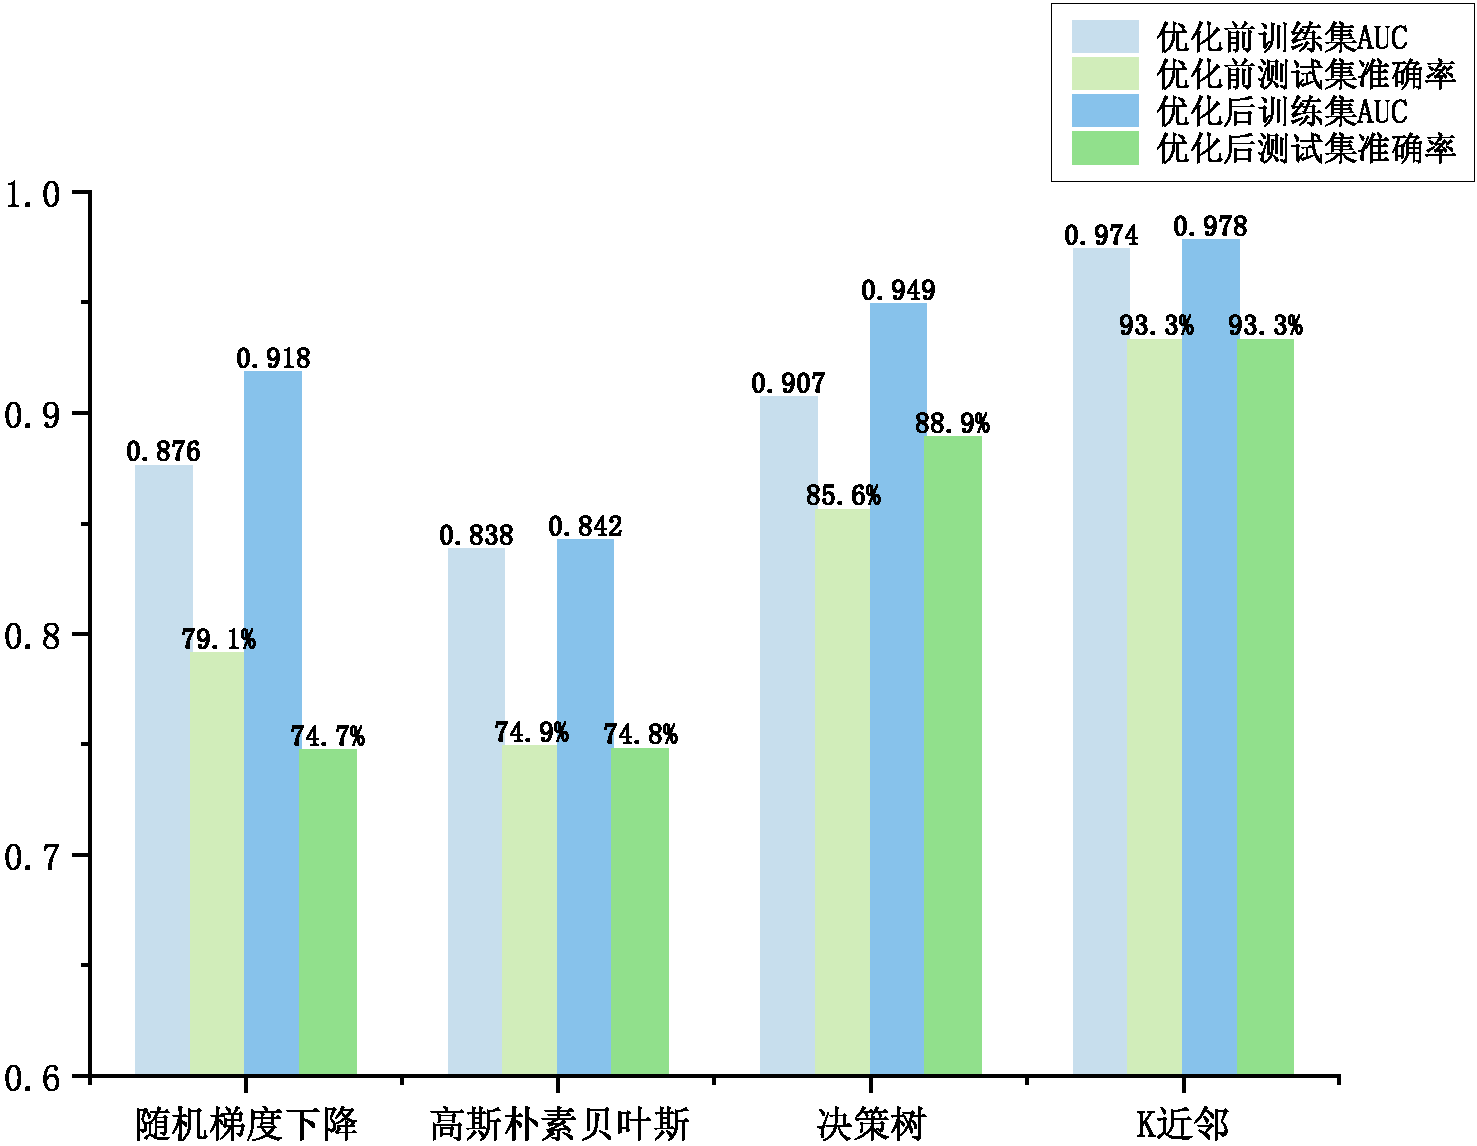
\includegraphics[width=.6\linewidth]{results/contrast_model}
      \caption[超参数调整前后模型性能对比]{\label{fig:contrast_model}超参数调整前后模型性能对比}
\end{figure}

\noindent
能模型及最佳模型下的的超参数组合。在进行超参数优化时通过网格搜索的方法来进行探索,需要设置好该算法的所有待调超参数的可选值集合,通过排列组合的方式得到该算法的多个实例,
在训练集上分别训练模型,使生成模型性能最好的超参数组合即为最优超参数。其中,判断模型性能最好的标准为该模型在训练集上的AUC数值大小。

\autoref{tab:super_para}展示了各算法模型超参数的搜索值域与最优超参数数值。其中,超参数值域加粗数值为默认超参数数值,最优超参数一栏则是在各模型在训练集AUC取最大值时使用的超参数组合。
而\autoref{fig:contrast_model}则展示了在超参数优化前后,训练模型在训练集上的AUC数值与模型在测试集上的准确率变化。其中,训练集上的数值进行了5层交叉验证后取得的平均值;测试集上的数值是在最优超参数时取得的。

从\autoref{fig:contrast_model}中的具体数值不难发现,四种模型的在超参数调整前后的AUC数值均有所提高。但只有决策树算法与K近邻算法
延续了之前的优秀表现,整体性能有微幅上升。但对随机梯度下降算法与高斯朴素贝叶斯算法而言,超参数的调整并没有明显的提升模型性能。
因此,本小节的结果进一步佐证了上小节初筛时得到的各项结论。


三、随机森林算法与特征降维

此前初筛过程中使用的均是单机器学习模型,本小节则使用了集成学习中的随机森林算法在新型时域波形描述特征集合上进行了模型训练。
\autoref{fig:dt_clf}展示了在随机森林构建的一棵决策树。在汇总所有决策树的结果表明,使用默认超参数生成的随机森林模型在训练集与测试集上均有着优秀的表现,
其在训练集上的AUC面积为0.990,在训练集与测试集上的准确率更是分别达到了95.2\%与97.0\%。
这些数值均高于之前的单机器模型中性能最好的K近邻算法与逻辑回归算法,充分体现了集成学习的优势。

另一方面,本章前文中阐述过随机森林算法可以用来衡量原始数据样本各属性的贡献度,并可进一步可以用作原始特征集的降维处理。在使用新型时域波形描述特征集的286个时域特征完成随机森林的构建之后,
计算各特征在随机森林中的平均深度即可得到各特征对最终模型的贡献度的数值,结果如\autoref{tab:rf_dr_1}所示。

\autoref{tab:rf_dr_1}列举了对随机森林累计贡献度达51.9\%的前36个特征。其中,基于脉搏波上升支的特征为红色背景填充,基于脉搏波下降支的特征为蓝色背景填充;特征名后的数字下标代表了
特征所对应的脉搏波位置,越靠近峰值的位置下标值越大。其中,贡献度最高的特征为$CVALF\_9$,贡献度为4.6\%。
若以特征$CVALF\_9$为基准,可以得到所有特征对随机森林模型的相对贡献度如\autoref{fig:rf_importance_pulse}所示。

在获取了所有特征对随机森林的贡献度后,此时即可按照贡献度按从高到低的顺序进行特征筛选。为评估筛选出的特征对子痫前期的识别能力,基于这些特征也应用随机

\begin{landscape}
      \begin{figure}[htbp]
            \centering
            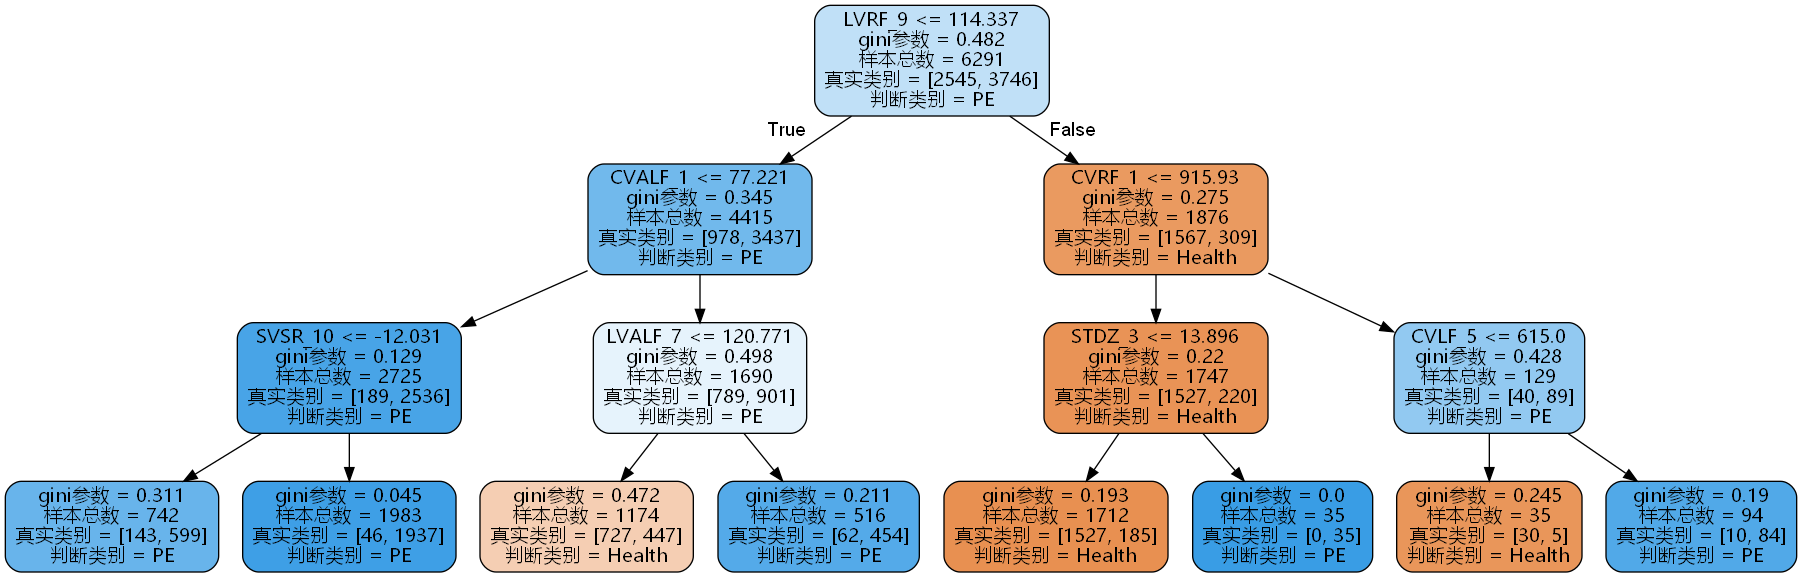
\includegraphics[width=\linewidth]{results/dt_clf}
            \caption{\label{fig:dt_clf}随机森林构建的一棵决策树示意}
      \end{figure}
\end{landscape}

\begin{center}
      \zihao{5}
      \begin{longtable}{m{2cm}<{\centering}m{2cm}<{\centering}m{2cm}<{\centering}m{2cm}<{\centering}m{2cm}<{\centering}m{2cm}<{\centering}}
            \caption[参与构建随机森林的特征贡献度(部分)]{参与构建随机森林的特征贡献度(部分)}\\
            \label{tab:rf_dr_1}\\
            \toprule
            \textbf{特征名}&\textbf{贡献度}&\textbf{特征名}&\textbf{贡献度}&\textbf{特征名}&\textbf{贡献度}\\
            \midrule
            \endfirsthead
            \caption[]{(续)}\\
            \midrule
            \textbf{特征名}&\textbf{贡献度}&\textbf{特征名}&\textbf{贡献度}&\textbf{特征名}&\textbf{贡献度}\\
            \midrule
            \endhead 
            \midrule
            \endfoot
            \bottomrule
            \endlastfoot
            \cellcolor{cyan}CVALF\_9                         & \cellcolor{cyan}4.6\%                            & \cellcolor{cyan}LVRF\_9                          & \cellcolor{cyan}3.4\%                            & SVD\_10                          & 3.0\%                            \\
            \cellcolor{cyan}SVAF\_10                         & \cellcolor{cyan}2.5\%                            & \cellcolor{cyan}LVALF\_7                         & \cellcolor{cyan}2.4\%                            & SVAT\_10                         & 2.3\%                            \\
            \cellcolor{cyan}CVRF\_11                         & \cellcolor{cyan}2.1\%                            & \cellcolor{pink}SVAR\_10                         & \cellcolor{pink}1.8\%                            & STDZ\_3                          & 1.6\%                            \\
            \cellcolor{cyan}LVRF\_8                          & \cellcolor{cyan}1.6\%                            & \cellcolor{cyan}LVALF\_6                         & \cellcolor{cyan}1.6\%                            & CVD\_11                          & 1.6\%                            \\
            STDZ\_1                                          & 1.5\%                                            & \cellcolor{cyan}CVALF\_8                         & \cellcolor{cyan}1.5\%                            & SVD\_9                           & 1.4\%                            \\
            \cellcolor{pink}SVAAR\_10                        & \cellcolor{pink}1.4\%                            & \cellcolor{cyan}CVALF\_1                         & \cellcolor{cyan}1.4\%                            & \cellcolor{pink}SVAAR\_8                         & \cellcolor{pink}1.3\%                            \\
            SVD\_8                                           & 1.1\%                                            & \cellcolor{pink}SVAR\_9                          & \cellcolor{pink}1.0\%                            & \cellcolor{cyan}SVAF\_9                          & \cellcolor{cyan}1.0\%                            \\
            \cellcolor{cyan}CVAAF\_1                         & \cellcolor{cyan}1.0\%                            & \cellcolor{cyan}LVLF\_8                          & \cellcolor{cyan}0.9\%                            & SVAT\_8                          & 0.9\%                            \\
            \cellcolor{cyan}CVRF\_1                          & \cellcolor{cyan}0.9\%                            & \cellcolor{cyan}CVAAF\_2                         & \cellcolor{cyan}0.9\%                            & \cellcolor{pink}SVAR\_8                          & \cellcolor{pink}0.8\%                            \\
            \cellcolor{cyan}SVAF\_2                          & \cellcolor{cyan}0.8\%                            & \cellcolor{pink}CVRR\_11                         & \cellcolor{pink}0.8\%                            & \cellcolor{cyan}LVRF\_1                          & \cellcolor{cyan}0.7\%                            \\
            \cellcolor{pink}SVSR\_7                          & \cellcolor{pink}0.7\%                            & \cellcolor{cyan}CVRF\_3                          & \cellcolor{cyan}0.7\%                            & \cellcolor{pink}CVALR\_10                        & \cellcolor{pink}0.7\%                            \\
            \cellcolor{cyan}CVALF\_7                         & \cellcolor{cyan}0.7\%                            & \cellcolor{pink}CVAAR\_5                         & \cellcolor{pink}0.7\%                            & \cellcolor{cyan}LVRF\_2                          & \cellcolor{cyan}0.6\%                           
      \end{longtable}
\end{center}

\begin{figure}[htbp]
      \centering
      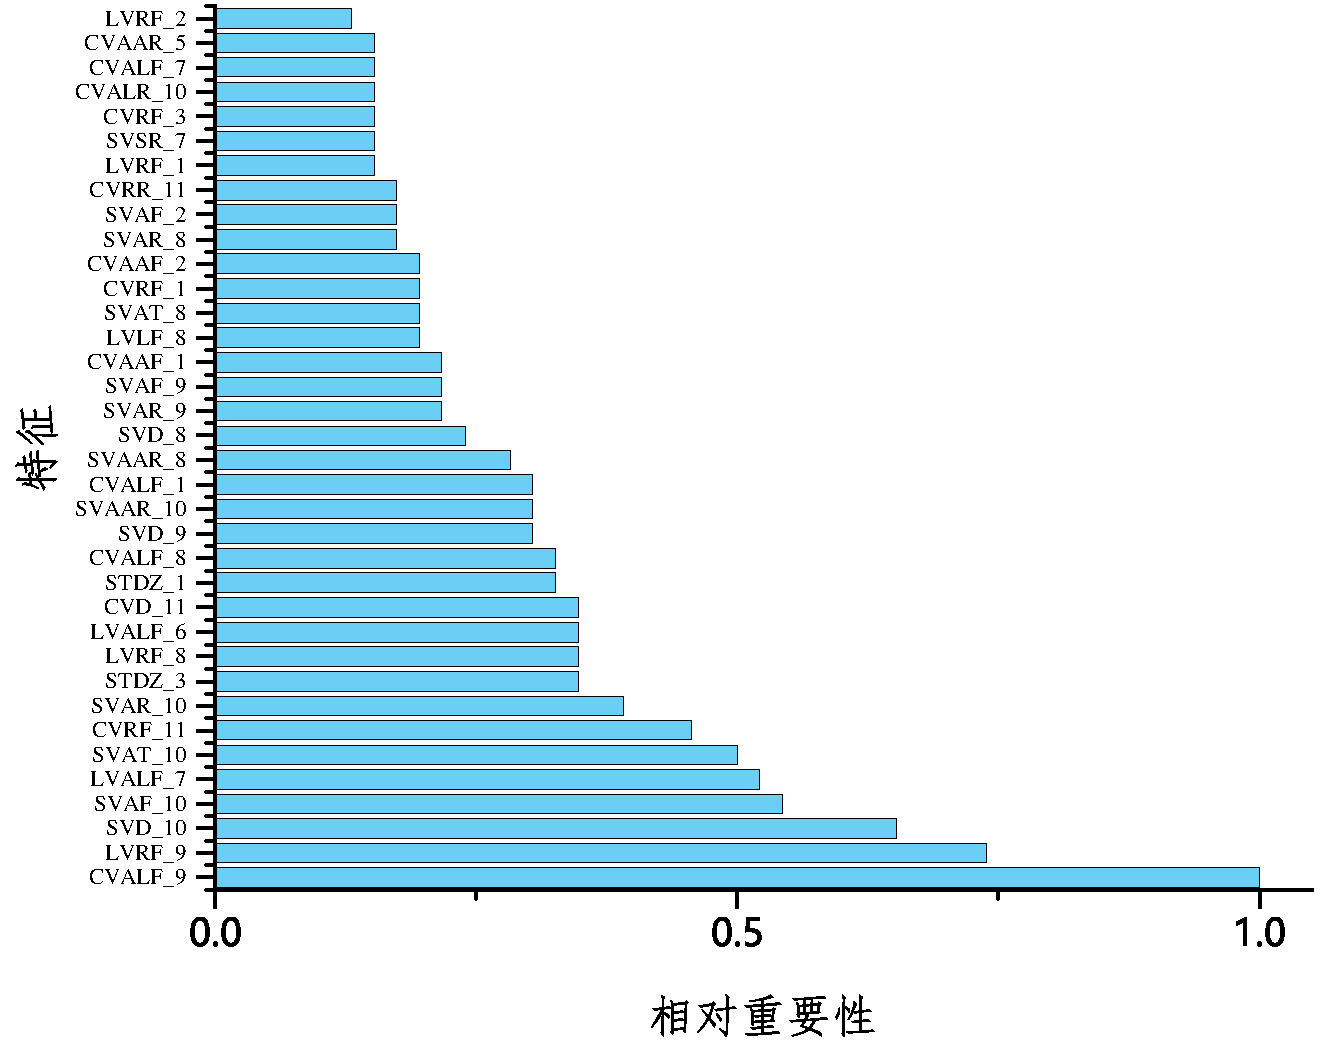
\includegraphics[width=0.55\linewidth]{results/rf_ip_pulse_0.52}
      \caption[各特征对随机森林的相对贡献度(局部)]{\label{fig:rf_importance_pulse}各特征对随机森林的相对贡献度(局部)}
\end{figure}

\noindent
森林算法建立模型并评估模型效果。\autoref{tab:rf_dr_2}展示了这一过程,
其中筛选按所有特征对初始随机森林贡献度的百分比例以10\%为梯度进行,每栏给出了使用筛选出的特征上建立的随机森林的效果。

\begin{landscape}
      \zihao{-5}
      \begin{longtable}{m{1.8cm}<{\centering}m{1.8cm}<{\centering}m{1.8cm}<{\centering}m{1.8cm}<{\centering}m{1.8cm}<{\centering}m{2cm}<{\centering}m{1cm}<{\centering}m{2cm}<{\centering}m{1cm}<{\centering}m{1cm}<{\centering}m{1cm}<{\centering}m{1cm}<{\centering}}
            \caption{随机森林对脉搏波特征降维效果}\\
            \label{tab:rf_dr_2}\\
            \toprule
            \multicolumn{3}{c}{\textbf{随机森林特征输入}}              & \multicolumn{2}{c}{\textbf{训练时间}} & \multicolumn{2}{c}{\textbf{训练集}} & \multicolumn{5}{c}{\textbf{测试集}}                                          \\
            \textbf{贡献度比例} & \textbf{特征数量} & \textbf{数量比例} & \textbf{训练时间}  & \textbf{时间比例}  & \textbf{混淆矩阵}   & \textbf{AUC}   & \textbf{混淆矩阵} & \textbf{精确率} & \textbf{召回率} & \textbf{F1值} & \textbf{准确率} \\
            \midrule
            \endfirsthead
            \caption[]{(续)}\\
            \midrule
            \multicolumn{3}{c}{\textbf{随机森林特征输入}}              & \multicolumn{2}{c}{\textbf{训练时间}} & \multicolumn{2}{c}{\textbf{训练集}} & \multicolumn{5}{c}{\textbf{测试集}}                                          \\
            \textbf{贡献度比例} & \textbf{特征数量} & \textbf{数量比例} & \textbf{训练时间}  & \textbf{时间比例}  & \textbf{混淆矩阵}   & \textbf{AUC}   & \textbf{混淆矩阵} & \textbf{精确率} & \textbf{召回率} & \textbf{F1值} & \textbf{准确率} \\
            \midrule
            \endhead 
            \midrule
            \endfoot
            \bottomrule
            \endlastfoot
            10.0\%         & 3             & 1.0\%         & 5.31           & 12.9\%           & $\left[ \begin{array}{cc} 2065 & 480 \\ 484 & 3262 \end{array} \right]$  & 0.931        & $\left[ \begin{array}{cc} 539 & 97 \\ 124 & 813 \end{array} \right]$  & 89.3\%       & 86.8\%       & 88.0\%       & 86.0\%       \\
            20.0\%         & 7             & 2.4\%         & 7.82           & 18.9\%           & $\left[ \begin{array}{cc} 2277 & 268 \\ 382 & 3364 \end{array} \right]$  & 0.961        & $\left[ \begin{array}{cc} 587 & 49 \\ 92 & 845 \end{array} \right]$   & 94.5\%       & 90.1\%       & 92.3\%       & 91.0\%       \\
            30.0\%         & 13            & 4.5\%         & 9.79           & 23.7\%           & $\left[ \begin{array}{cc} 2422 & 123 \\ 200 & 3546 \end{array} \right]$  & 0.987        & $\left[ \begin{array}{cc} 612 & 24 \\ 34 & 903 \end{array} \right]$   & 97.4\%       & 96.4\%       & 96.9\%       & 96.3\%       \\
            40.0\%         & 21            & 7.3\%         & 11.90          & 28.8\%           & $\left[ \begin{array}{cc} 2432 & 113 \\ 145 & 3601 \end{array} \right]$  & 0.993        & $\left[ \begin{array}{cc} 615 & 21 \\ 30 & 907 \end{array} \right]$   & 97.7\%       & 96.8\%       & 97.3\%       & 96.8\%       \\
            50.0\%         & 34            & 11.9\%        & 15.17          & 36.7\%           & $\left[ \begin{array}{cc} 2433 & 112 \\ 146 & 3600 \end{array} \right]$  & 0.993        & $\left[ \begin{array}{cc} 616 & 20 \\ 28 & 909 \end{array} \right]$   & 97.8\%       & 97.0\%       & 97.4\%       & 97.0\%       \\
            60.0\%         & 51            & 17.8\%        & 20.91          & 50.6\%           & $\left[ \begin{array}{cc} 2442 & 103 \\ 115 & 3631 \end{array} \right]$  & 0.994        & $\left[ \begin{array}{cc} 620 & 16 \\ 27 & 910 \end{array} \right]$   & 98.3\%       & 97.1\%       & 97.7\%       & 97.3\%       \\
            70.0\%         & 74            & 25.9\%        & 23.67          & 57.3\%           & $\left[ \begin{array}{cc} 2431 & 114 \\ 125 & 3621 \end{array} \right]$  & 0.993        & $\left[ \begin{array}{cc} 618 & 18 \\ 23 & 914 \end{array} \right]$   & 98.1\%       & 97.5\%       & 97.8\%       & 97.4\%       \\
            80.0\%         & 108           & 37.8\%        & 29.33          & 71.0\%           & $\left[ \begin{array}{cc} 2431 & 114 \\ 130 & 3616 \end{array} \right]$  & 0.993        & $\left[ \begin{array}{cc} 615 & 21 \\ 26 & 911 \end{array} \right]$   & 97.7\%       & 97.2\%       & 97.5\%       & 97.0\%       \\
            90.0\%         & 162           & 56.6\%        & 38.11          & 92.3\%           & $\left[ \begin{array}{cc} 2421 & 124 \\ 134 & 3612 \end{array} \right]$  & 0.991        & $\left[ \begin{array}{cc} 619 & 17 \\ 25 & 912 \end{array} \right]$   & 98.1\%       & 97.3\%       & 97.8\%       & 97.3\%       \\
            100.0\%        & 286           & 100.0\%       & 41.30          & 100.0\%          & $\left[ \begin{array}{cc} 2404 & 141 \\ 160 & 3586 \end{array} \right]$  & 0.990        & $\left[ \begin{array}{cc} 617 & 19 \\ 28 & 909 \end{array} \right]$   & 98.0\%       & 97.0\%       & 97.5\%       & 97.0\%       \\
      \end{longtable}
\end{landscape}


从上述特征降维处理过程中可以得到以下结论:

1、本研究提出的新型时域波形描述特征集中包含了具有一定能力的表征子痫前期特征。新型时域波形描述特征集共有286个特征中,其平均贡献度为0.34\%,而贡献度最高的单特征CVALF\_9的贡献度为平均值的13.5倍。

2、从\autoref{tab:rf_dr_1}中各特征具体的贡献度可以发现,与下降支相关的特征要远多于上升支的特征。这也与脉搏波下降支是血液回流过程的反应、下降支包含了更多的血液循环中细节信息的事实相符合。

3、从\autoref{tab:rf_dr_1}的指标种类来看,左视类指标相较中视类指标与分层类指标也更少。这可能与左视类指标对下降支的表征效果不及另外两类有关。

4、从\autoref{tab:rf_dr_1}中的特征的下标来看,贡献度较高的特征主要集中在前端(1-3)与尾端(8-10)。这说明脉搏波下降支的前端与尾端可能包含了更多与子痫前期相关的信息。

5、从\autoref{tab:rf_dr_2}的训练过程来看,随着特征数量的减少,随机森林模型的训练速度大大加快。其次,随着特征数量的减少,新生成的随机森林模型在训练集与测试集上均出现了性能小幅提高再下降的整体趋势,
模型最佳性能出现在贡献度60\%-70\%之间。这说明筛选刚开始进行时排除了大量无关特征,从而使模型性能得到了提升;而随着筛选的进行,对模型生成有贡献度的特征数量的也在减少,导致随机森林的性能降低。

6、从\autoref{tab:rf_dr_2}的训练效果来看,新型时域波形描述特征集的286个特征中具有子痫前期表征能力的特征较少,存在大量不具任何子痫前期表征能力的冗余特征。在保留原始特征集90\%的贡献度的条件下,就可以
在几乎不损失模型预测能力的条件下排除约43.4\%的无关特征。甚至在仅保留原始特征集30\%的贡献度的13个特征上建立的随机森林模型也有着接近原始随机森林模型的性能(准确率96.3\% VS 97.0\%)。

\subsection{按照被试人员分层抽样}

第四章已经在数据集划分时阐述过,将原始数据集按照被试分层抽样可以更加客观评估模型的泛化能力。按这种方式,将63名被试孕妇的全部脉搏波波形被划分为训练集,余下16名被试的全波波形被划分为测试集,
并使用了在上小节中表现较好的K近
邻、决策树及随机森林等三种算法在新划分的训练集上进行子痫前期识别模型的训练。这三种模型的具体表现如\autoref{tab:model_screen2}所示,其中,训练集上的AUC数值是在进行了5层交叉验证后取得的。

\begin{landscape}
      \zihao{-5}
      \begin{longtable}{m{3cm}<{\centering}m{1.7cm}<{\centering}m{2.3cm}<{\centering}m{1cm}<{\centering}m{1cm}<{\centering}m{1cm}<{\centering}m{1cm}<{\centering}m{1cm}<{\centering}m{2cm}<{\centering}m{1cm}<{\centering}m{1cm}<{\centering}m{1cm}<{\centering}m{1cm}<{\centering}}
            \caption{几种机器学习模型在被试人员分层抽样的数据集上的表现}\\
            \label{tab:model_screen2}\\
            \toprule
            &  & \multicolumn{6}{c}{\textbf{训练集}} & \multicolumn{5}{c}{\textbf{验证集}}                                                                                                                                                                                                      \\
            \multirow{-2}{*}{\textbf{模型类型}} & \multirow{-2}{*}{\textbf{训练时间}} & \textbf{混淆矩阵} &  \textbf{精确率} &  \textbf{召回率} &  \textbf{F1值} &  \textbf{准确率} &  \textbf{AUC} &  \textbf{混淆矩阵} &  \textbf{精确率} &  \textbf{召回率} &  \textbf{F1值} &  \textbf{准确率}    \\
            \midrule
            \endfirsthead
            \caption[]{(续)}\\
            \midrule
            &  & \multicolumn{6}{c}{\textbf{训练集}} & \multicolumn{5}{c}{\textbf{验证集}}                                                                                                                                                                                                      \\
            \multirow{-2}{*}{\textbf{模型类型}} & \multirow{-2}{*}{\textbf{训练时间}} & \textbf{混淆矩阵} &  \textbf{精确率} &  \textbf{召回率} &  \textbf{F1值} &  \textbf{准确率} &  \textbf{AUC} &  \textbf{混淆矩阵} &  \textbf{精确率} &  \textbf{召回率} &  \textbf{F1值} &  \textbf{准确率}    \\
            \midrule
            \endhead 
            \midrule
            \endfoot
            \bottomrule
            \endlastfoot
            K近邻算法      &   4.08 s  &     $\left[ \begin{array}{cc} 2250 & 384 \\ 888 & 2815 \end{array} \right]$ & 88.0\% & 76.0\% &81.6\% & 80.0\% & 0.870 &
            $\left[ \begin{array}{cc} 357 & 190 \\ 141 & 839 \end{array} \right]$ & 81.5\% & 85.6\% & 83.5\% & 78.3\% \\
            决策树算法      &   1.44 s  &     $\left[ \begin{array}{cc} 2062 & 572 \\ 706 & 2997 \end{array} \right]$ & 84.0\% & 80.9\% & 82.4\% & 79.8\% & 0.862 &
            $\left[ \begin{array}{cc} 168 & 379 \\ 136 & 844 \end{array} \right]$ & 69.0\% & 86.1\% & 76.6\% & 66.3\% \\
            随机森林算法      &   50.03 s  &     $\left[ \begin{array}{cc} 2326 & 308 \\ 718 & 2985 \end{array} \right]$ & 90.6\% & 80.6\% & 85.3\% & 83.8\% & 0.929 &
            $\left[ \begin{array}{cc} 317 & 230 \\ 89 & 891 \end{array} \right]$ & 79.5\% & 90.9\% & 84.8\% & 79.1\% \\
      \end{longtable}
\end{landscape}

\begin{landscape}
      \zihao{-5}
      \begin{longtable}{m{2cm}<{\centering}m{2cm}<{\centering}m{2cm}<{\centering}m{2cm}<{\centering}m{2cm}<{\centering}m{2cm}<{\centering}m{2cm}<{\centering}m{2cm}<{\centering}m{2cm}<{\centering}}
            \caption{几种机器学习模型按被试统计后的性能表现}\\
            \label{tab:model_detail}\\
            \toprule
            \multirow{2}{*}{\textbf{被试孕妇}} & \multirow{2}{*}{\textbf{波形总数}} & \multicolumn{2}{c}{\textbf{K近邻算法}} & \multicolumn{2}{c}{\textbf{决策树}} & \multicolumn{2}{c}{\textbf{随机森林}} & \multirow{2}{*}{\begin{tabular}[c]{@{}l@{}}\textbf{真实子痫前}\\ \textbf{期患病状态}\end{tabular}} \\
                        &                       & \textbf{预测阳性数目}     & \textbf{预测比例}       & \textbf{预测阳性数目}     & \textbf{预测比例}       & \textbf{预测阳性数目}     & \textbf{预测比例}        &                                                                        \\
            \midrule
            \endfirsthead
            \caption[]{(续)}\\
            \midrule
            \multirow{2}{*}{\textbf{被试孕妇}} & \multirow{2}{*}{\textbf{波形总数}} & \multicolumn{2}{c}{\textbf{K近邻算法}} & \multicolumn{2}{c}{\textbf{决策树}} & \multicolumn{2}{c}{\textbf{随机森林}} & \multirow{2}{*}{\begin{tabular}[c]{@{}l@{}}\textbf{真实子痫前}\\ \textbf{期患病状态}\end{tabular}} \\
                        &                       & \textbf{预测阳性数目}     & \textbf{预测比例}       & \textbf{预测阳性数目}     & \textbf{预测比例}       & \textbf{预测阳性数目}     & \textbf{预测比例}        &                                                                        \\
            \midrule
            \endhead 
            \midrule
            \endfoot
            \bottomrule
            \endlastfoot
            cmf                   & 88                    & 54         & 61.4\%     & 85         & 96.6\%     & 53         & 60.2\%      & 0                                                                      \\
            lxx                   & 63                    & 32         & 50.8\%     & 53         & 84.1\%     & 34         & 54.0\%      & 0                                                                      \\
            shs                   & 112                   & 37         & 33.0\%     & 105        & 93.8\%     & 55         & 49.1\%      & 0                                                                      \\
            sxh                   & 95                    & 27         & 28.4\%     & 64         & 67.4\%     & 21         & 22.1\%      & 0                                                                      \\
            wdq                   & 36                    & 0          & 0.0\%      & 0          & 0.0\%      & 0          & 0.0\%       & 0                                                                      \\
            wsj                   & 78                    & 0          & 0.0\%      & 2          & 2.6\%      & 0          & 0.0\%       & 0                                                                      \\
            ygy                   & 75                    & 40         & 53.3\%     & 70         & 93.3\%     & 67         & 89.3\%      & 0                                                                      \\
            gmn                   & 139                   & 106        & 76.3\%     & 135        & 97.1\%     & 109        & 78.4\%      & 1                                                                      \\
            ty                    & 98                    & 97         & 99.0\%     & 97         & 99.0\%     & 97         & 99.0\%      & 1                                                                      \\
            wjh                   & 86                    & 86         & 100.0\%    & 86         & 100.0\%    & 86         & 100.0\%     & 1                                                                      \\
            xjf                   & 106                   & 23         & 21.7\%     & 59         & 55.7\%     & 87         & 82.1\%      & 1                                                                      \\
            ywy                   & 111                   & 110        & 99.1\%     & 111        & 100.0\%    & 111        & 100.0\%     & 1                                                                      \\
            yxl                   & 110                   & 110        & 100.0\%    & 108        & 98.2\%     & 110        & 100.0\%     & 1                                                                      \\
            zdq                   & 89                    & 81         & 91.0\%     & 84         & 94.4\%     & 82         & 92.1\%      & 1                                                                      \\
            zl                    & 152                   & 137        & 90.1\%     & 75         & 49.3\%     & 120        & 78.9\%      & 1                                                                      \\
            zyy                   & 89                    & 89         & 100.0\%    & 89         & 100.0\%    & 89         & 100.0\%     & 1                                                                       \\    
      \end{longtable}
\end{landscape}


横向对比\autoref{tab:model_screen}、\autoref{tab:rf_dr_2}及\autoref{tab:model_screen2}中结果可以发现,在将原始数据按被试人员分层抽样之后,K近邻、决策树及随机森林等三种算法在训练集与测试集上的均出现了
较为明显的性能下降,在测试集上性能下降得尤为明显。而单就\autoref{tab:model_screen2}而言,随机森林算法与K近邻算法的性能接近,在测试集上F1值可达到83\%以上,准确率也在78\%以上;决策树算法表现最差F1值仅有76.6\%,准确率也仅有66.3\%。

注意到\autoref{tab:model_screen2}中结果仍是按照脉搏波波形进行统计,并不能完全反应按被试分层抽样的结果。将\autoref{tab:model_screen2}各模型在测试集上的所有波形的预测结果,按是否隶属同一被试分类进行统计后如\autoref{tab:model_detail}所示。
\autoref{tab:model_detail}给出了每名被试所对应的脉搏波波形总数,并统计了使用K近邻、决策树及随机森林等三种算法生成的预测模型预测为子痫前期阳性的脉搏波波形数目,而预测比例一栏则为预测为阳性的脉搏波波形数目与该被试脉搏波波形总数之比。
最后,\autoref{tab:model_detail}也给出了每名被试所对应的子痫前期真实患病状态。

\begin{figure}[htbp]
      \centering
      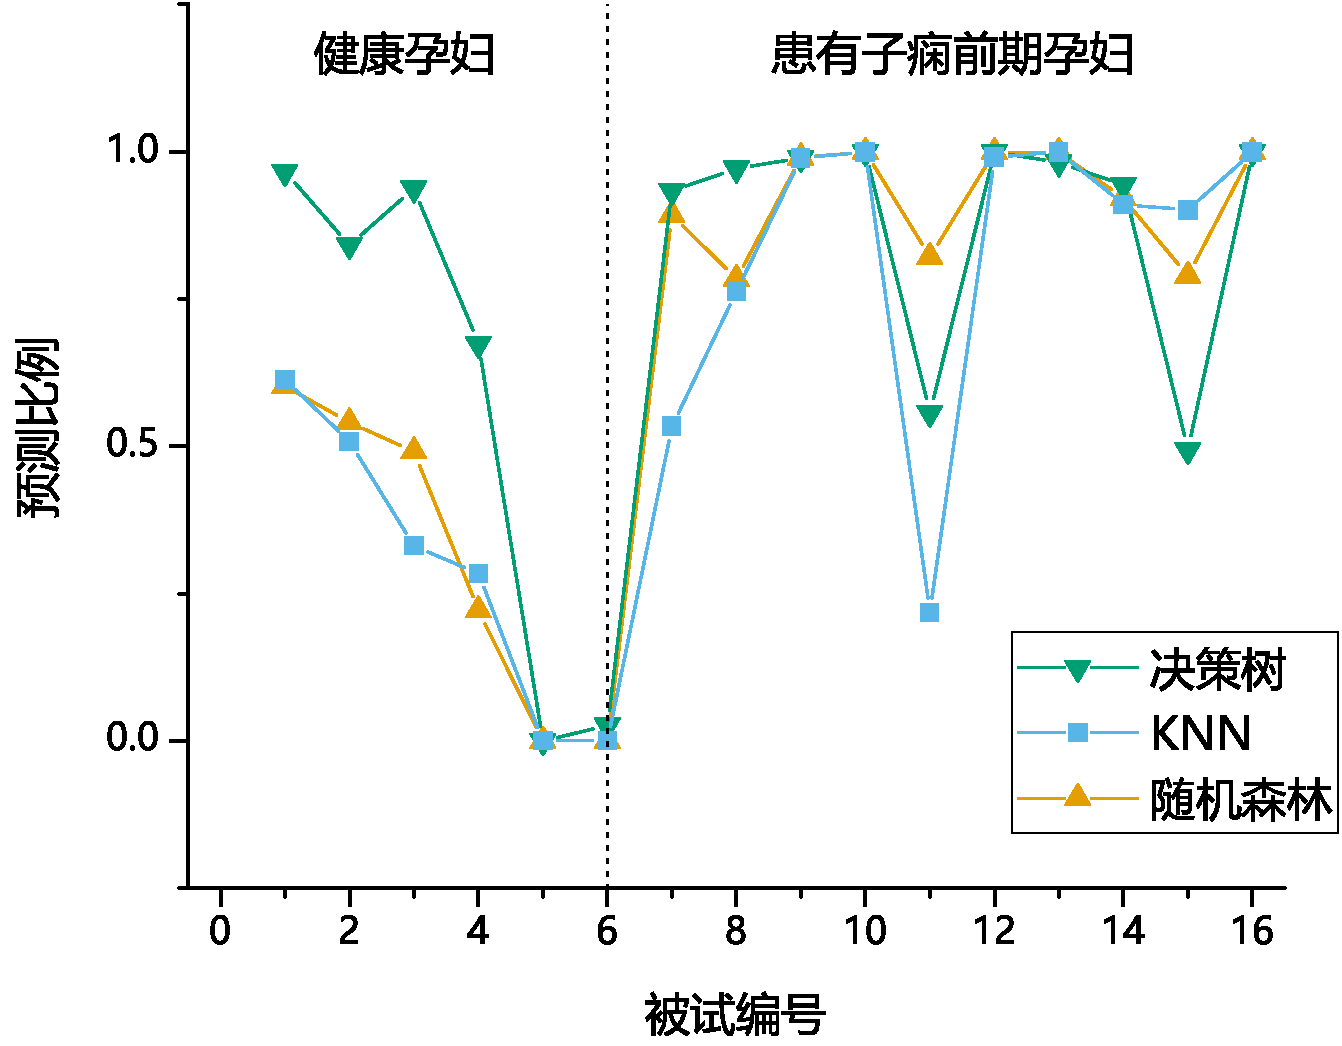
\includegraphics[width=.55\linewidth]{results/detail}
      \caption[基于三种算法得到的子痫前期预测比例散点图]{\label{fig:model_detail}基于三种算法得到的子痫前期预测比例散点图}
\end{figure}

在\autoref{tab:model_detail}的基础上,将三种算法训练所得的模型在测试集上的预测比例作为该模型表征被试子痫前期患病状态的输出,则可以得到\autoref{fig:model_detail}所示的散点图。此时,对子痫前期的识别分析可以转换为寻找
能将\autoref{fig:model_detail}进行最佳分割的阈值。遍历各模型的预测比例数值并将该数值作为分割阈值,可以得到在该数值下的混淆矩阵,并进一步得到该数值对应的敏感性与特异性。最终,三种模型的预测比例
所对应的ROC曲线如\autoref{fig:model_roc}所示。其中,决策树、K近邻及随机森林三种模型对应的AUC数值分别为0.825、0.921及0.952。同时,借助约登指数可以确定三种模型的最佳分割阈值分别为0.969、0.907与0.688,各模型在最佳阈值下的
混淆矩阵如\autoref{tab:cm_on_best}所示。三种模型的整体识别准确率分别为81.3\%、81.3\%与93.8\%。

\begin{figure}[htbp]
      \centering
      \includegraphics[width=.6\linewidth]{results/roc}
      \caption[由子痫前期预测比例得到的ROC曲线]{\label{fig:model_roc}由子痫前期预测比例得到的ROC曲线}
\end{figure}
\begin{table}[htbp]
      \zihao{5}
      \centering
      \caption{\label{tab:cm_on_best}三种模型在最佳分割阈值下的混淆矩阵}
      \begin{tabular}{ccc}
      \toprule
      \textbf{决策树算法}&\textbf{K近邻算法}&\textbf{随机森林算法}\\
      \midrule
      $\left[ \begin{array}{cc} 6 & 3 \\ 0 & 7 \end{array} \right]$ & $\left[ \begin{array}{cc} 6 & 3 \\ 0 & 7 \end{array} \right]$ & $\left[ \begin{array}{cc} 9 & 0 \\ 1 & 6 \end{array} \right]$ \\
      \bottomrule
      \end{tabular}%
\end{table}%

从上述研究结果中可以得到以下结论:

1、在按被试划分原始数据集后,再进行子痫前期识别模型的训练,所得的子痫前期预测比例具有较好的子痫前期识别能力。借助AUC与ROC分析,三种算法可以分别达到81.3\%、81.3\%与93.8\%的整体准确率。

2、从\autoref{fig:model_roc}来看,在K近邻、决策树及随机森林等三种分类算法构建的识别模型中,随机森林模型有着最佳的分类效果。其AUC数值最大,为0.952。

3、从\autoref{tab:cm_on_best}来看,随机森林算法识别的总体准确率高于决策树与K近邻算法,且识别为假阴性的数目(0)也少于其他两种模型(3与3)。

4、从最佳分割阈值来看,决策树与K近邻算法的预测比例分割阈值(0.969与0.907)过于接近100\%,有泛化能力不足的潜在风险,而随机森林模型的分割阈值(0.688)则相对适中。

\section{基于脉搏波原始采样点生成的模型及分析}

基于脉搏波原始采样点,本小节也进行了与上小节类似的研究工作,分别按波形与被试对脉搏波波形进行了处理与建模。

\subsection{按照全部波形抽样}

一、模型初筛

本部分沿用了上小节中的结论,直接选取了决策树、K近邻及随机森林等三种算法来进行子痫前期识别模型的研究。使用这三种算法在脉搏波原始采样点按照全部波形分层抽样所得的数据集上的表现如
\autoref{tab:model_screen3}所示。其中,三种模型在训练集相关数据是对原始训练集数据经过5层交叉验证后得到的;决策树与K近邻模型的数据已经是经行过超参数调优后的结果;表格中处理方式一栏的补零与重采样对应第四章中所介绍
的对脉搏波原始采样点的两种处理策略。

从\autoref{tab:model_screen3}可以得到以下结论:

1、在测试集上,从模型方面来看,K近邻模型构建速度最快,随机森林处理速度最慢。而从模型分类效果来看,三种模型在测试集上的AUC数值均超过了0.900,其中随机森林的AUC数值更是在0.967以上。
在精度­召回率权衡上,K近邻与随机森林算法明显优于决策树算法,精确率、召回率及F1 数值均在 90.0\% 附近或以上。

2、在验证集上,K近邻与随机森林算法的泛化能力也同样优于决策树算法。就准确率而言,K近邻与随机森林算法均在91\%以上,而决策树算法则不足87\%。
在精度­召回率权衡上,K近邻与随机森林算法明显优于决策树算法,精确率、召回率及F1 数值均在 90.0\% 。

3、横向对比两种对脉搏波波形进行对齐的处理方式可以发现,直接在脉搏波尾端进行补零处理会使各模型在构建速度、训练集AUC及模型整体准确率、精确率等方面均略微优于对脉搏波重采样处理的相应数据。

二、采样点贡献度

与上小节中处理类似,在脉搏波原始采样点上使用随机森林构建模型后,可以得到
原始脉搏波中不同位置上的采样点对最终随机森林模型的贡献度。但基于贡献度对采样点的降维处理
缺乏实际处理的意义,本研究未进行相应的处理分析工作。

\begin{landscape}
      \zihao{-5}
      \begin{longtable}{m{1.5cm}<{\centering}m{1.5cm}<{\centering}m{1.5cm}<{\centering}m{2cm}<{\centering}m{1cm}<{\centering}m{1cm}<{\centering}m{1cm}<{\centering}m{1cm}<{\centering}m{1cm}<{\centering}m{2cm}<{\centering}m{1cm}<{\centering}m{1cm}<{\centering}m{1cm}<{\centering}m{1cm}<{\centering}}
            \caption{基于脉搏波原始采样点的识别模型的初筛结果}\\
            \label{tab:model_screen3}\\
            \toprule
                  & \multicolumn{1}{c}{}   & \multicolumn{1}{c}{}  & \multicolumn{6}{c}{\textbf{训练集(5层交叉验证)}}   & \multicolumn{5}{c}{\textbf{验证集}}     \\
            \multirow{-2}{*}{\textbf{处理方式}}  & \multicolumn{1}{c}{\multirow{-2}{*}{\textbf{模型类型}}} & \multicolumn{1}{c}{\multirow{-2}{*}{\textbf{训练时间}}} & \textbf{混淆矩阵} & \textbf{精确率} & \textbf{召回率}& \textbf{F1值} & \textbf{准确率}& \textbf{AUC} & \textbf{混淆矩阵}& \textbf{精确率} & \textbf{召回率} & \textbf{F1值}& \textbf{准确率} \\
            \midrule
            \endfirsthead
            \caption[]{(续)}\\
            \midrule
                  & \multicolumn{1}{c}{}   & \multicolumn{1}{c}{}  & \multicolumn{6}{c}{\textbf{训练集(5层交叉验证)}}   & \multicolumn{5}{c}{\textbf{验证集}}                                                                                                                                                                                                    \\
            \multirow{-2}{*}{\textbf{处理方式}}  & \multicolumn{1}{c}{\multirow{-2}{*}{\textbf{模型类型}}} & \multicolumn{1}{c}{\multirow{-2}{*}{\textbf{训练时间}}} & \textbf{混淆矩阵} & \textbf{精确率} & \textbf{召回率}& \textbf{F1值} & \textbf{准确率}& \textbf{AUC} & \textbf{混淆矩阵}& \textbf{精确率} & \textbf{召回率} & \textbf{F1值}& \textbf{准确率} \\
            \midrule
            \endhead 
            \midrule
            \endfoot
            \bottomrule
            \endlastfoot
            & 决策树      & 4.13    & $\left[ \begin{array}{cc} 1906 & 639 \\ 428 & 3318 \end{array} \right]$ & 83.9\%  & 88.6\%  & 86.1\% & 83.0\% & 0.914    & $\left[ \begin{array}{cc} 504 & 132 \\ 85 & 852 \end{array} \right]$ & 86.6\%  & 90.9\%  & 88.7\% & 86.2\% \\
            & K近邻     & 2.81    & $\left[ \begin{array}{cc} 2309 & 236 \\ 392 & 3354 \end{array} \right]$ & 93.4\%  & 90.0\%  & 91.4\% & 90.0\%   & 0.967  & $\left[ \begin{array}{cc} 587 & 49 \\ 87 & 850 \end{array} \right]$ & 94.5\%   & 90.7\%   & 92.6\% & 91.4\% \\
            \multirow{-3}{*}{补零} & 随机森林    & 23.23    & $\left[ \begin{array}{cc} 2295 & 250 \\ 271 & 3475 \end{array} \right]$ & 93.3\%  & 92.8\% & 93.0\% & 91.7\%  & 0.977 & $\left[ \begin{array}{cc} 587 & 49 \\ 52 & 885 \end{array} \right]$  & 94.8\% & 94.5\%   & 94.6\% & 93.6\% \\
            & 决策树      & 6.77    & $\left[ \begin{array}{cc} 2206 & 539 \\ 554 & 3192 \end{array} \right]$ & 85.6\%  & 85.2\%  & 85.4\% & 82.6\% & 0.902    & $\left[ \begin{array}{cc} 532 & 104 \\ 149 & 788 \end{array} \right]$ & 88.3\%  & 84.1\%  & 86.2\% & 83.9\% \\
            & K近邻     & 3.90    & $\left[ \begin{array}{cc} 2234 & 311 \\ 392 & 3354 \end{array} \right]$ & 91.5\%  & 89.5\%  & 90.5\% & 88.8\%   & 0.957 & $\left[ \begin{array}{cc} 583 & 53 \\ 79 & 858 \end{array} \right]$ & 94.2\%   & 91.2\%   & 92.9\% & 91.6\% \\
            \multirow{-3}{*}{重采样} & 随机森林    & 51.57    & $\left[ \begin{array}{cc} 2222 & 323 \\ 305 & 3441 \end{array} \right]$ & 91.4\%  & 91.9\% & 91.6\% & 90.0\%  & 0.967 & $\left[ \begin{array}{cc} 574 & 62 \\ 56 & 881 \end{array} \right]$  & 93.4\% & 94.0\%   & 93.7\% & 92.5\% \\
      \end{longtable}
\end{landscape}

\autoref{fig:rf_imp2}展示了\autoref{tab:model_screen3}中基于两种脉搏波对齐方式得到随机森林模型中各采样点的贡献度,此外,\autoref{fig:rf_imp2}
也给出了所有脉搏波波形两种对齐方式得到的“平均脉搏波”波形示意(即所有脉搏波波形的按采样点进行算术平均再归一化后所得的结果)。

\begin{figure}[htbp]
      \centering
      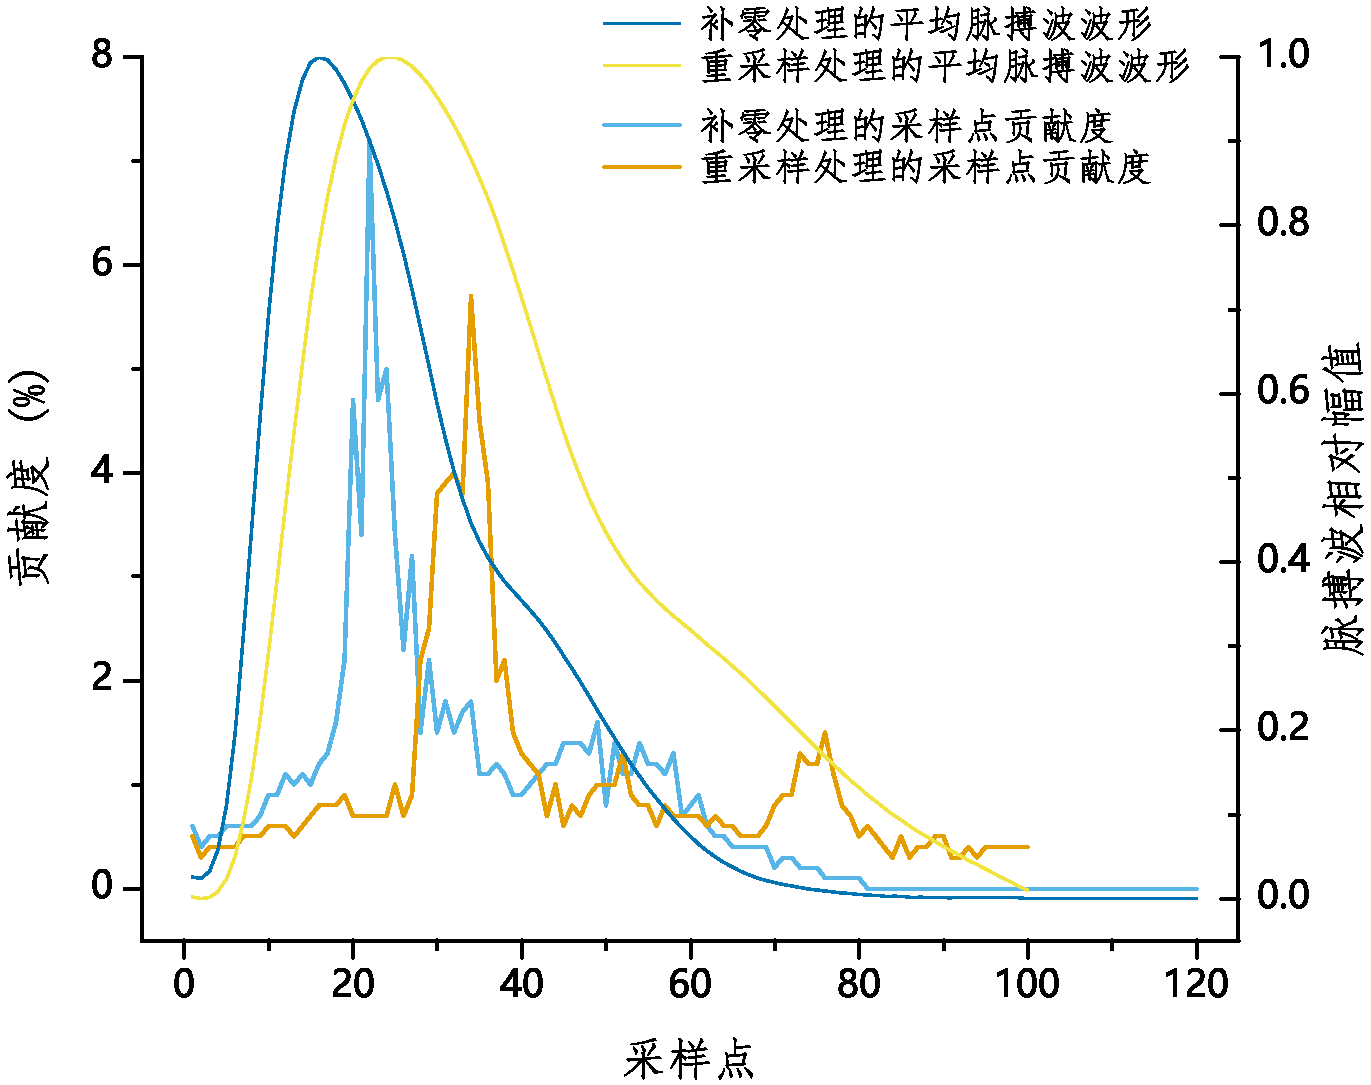
\includegraphics[width=.6\linewidth]{results/rf_imp2}
      \caption{\label{fig:rf_imp2}脉搏波采样点对随机森林的贡献度}
\end{figure}

从\autoref{fig:rf_imp2}可以得到以下结论:

1、按照两种方式处理得到的采样点贡献度分布形态上高度相似,均是在平均脉搏波的波峰之后出现贡献度的主峰,在平均脉搏波的下降支尾端附近出现第二个次峰。

2、尽管补零处理的方式具有更多的采样点数(120个),但采样点贡献度的分布更为集中,各有效特征点的贡献度数值更大。在\autoref{fig:rf_imp2}中进行补零处理的80以后的采样点几乎完全没有参与
最终随机森林模型的构建。而采样点为80则对应着本研究中得到的大多数脉搏波波形时间的最大值。因此,在逻辑上这些新值及原始采样值中采样点80以后的数据均属于冗余项。

\subsection{按照被试人员分层抽样}

本小节在脉搏波原始采样点的基础上,按照被试人员分层抽样划分了训练集与测试集,采用了K近邻、决策树及随机森林等三种算法构建了子痫前期的识别分类模型。
这三种模型的具体表现如\autoref{tab:model_screen4}所示。其中,训练集上的AUC数值是在进行了5层交叉验证后取得的。

从\autoref{tab:model_screen4}中可以得到以下结论:

\begin{landscape}
      \zihao{6}
      \begin{longtable}{m{1.5cm}<{\centering}m{1.5cm}<{\centering}m{1.5cm}<{\centering}m{2cm}<{\centering}m{1cm}<{\centering}m{1cm}<{\centering}m{1cm}<{\centering}m{1cm}<{\centering}m{1cm}<{\centering}m{2cm}<{\centering}m{1cm}<{\centering}m{1cm}<{\centering}m{1cm}<{\centering}m{1cm}<{\centering}}
            \caption{几种机器学习模型在被试人员分层抽样的数据集上的表现}\\
            \label{tab:model_screen4}\\
            \toprule
            &     &  & \multicolumn{6}{c}{\textbf{训练集}} & \multicolumn{5}{c}{\textbf{验证集}}                                                                                                                                                                                                      \\
            \multirow{-2}{*}{\textbf{处理方式}}&\multirow{-2}{*}{\textbf{模型类型}} & \multirow{-2}{*}{\textbf{训练时间}} & \textbf{混淆矩阵} &  \textbf{精确率} &  \textbf{召回率} &  \textbf{F1值} &  \textbf{准确率} &  \textbf{AUC} &  \textbf{混淆矩阵} &  \textbf{精确率} &  \textbf{召回率} &  \textbf{F1值} &  \textbf{准确率}    \\
            \midrule
            \endfirsthead
            \caption[]{(续)}\\
            \midrule
            &     &  & \multicolumn{6}{c}{\textbf{训练集}} & \multicolumn{5}{c}{\textbf{验证集}}                                                                                                                                                                                                      \\
            \multirow{-2}{*}{\textbf{处理方式}}&\multirow{-2}{*}{\textbf{模型类型}} & \multirow{-2}{*}{\textbf{训练时间}} & \textbf{混淆矩阵} &  \textbf{精确率} &  \textbf{召回率} &  \textbf{F1值} &  \textbf{准确率} &  \textbf{AUC} &  \textbf{混淆矩阵} &  \textbf{精确率} &  \textbf{召回率} &  \textbf{F1值} &  \textbf{准确率}    \\
            \midrule
            \endhead 
            \midrule
            \endfoot
            \bottomrule
            \endlastfoot
            &     K近邻算法      &   3.12 s  &     $\left[ \begin{array}{cc} 2191 & 443 \\ 974 & 2729 \end{array} \right]$ & 86.0\% & 73.7\% &79.4\% & 77.6\% & 0.863 &
            $\left[ \begin{array}{cc} 357 & 190 \\ 141 & 839 \end{array} \right]$ & 81.5\% & 85.6\% & 83.5\% & 78.3\% \\
            &     决策树算法      &   3.62 s  &     $\left[ \begin{array}{cc} 2056 & 578 \\ 659 & 3044 \end{array} \right]$ & 84.0\% & 82.2\% & 83.1\% & 80.5\% & 0.880 &
            $\left[ \begin{array}{cc} 202 & 345 \\ 151 & 829 \end{array} \right]$ & 70.6\% & 84.6\% & 77.0\% & 67.5\% \\
            \multirow{-3}{*}{补零}  & 随机森林算法      &   23.18 s  &     $\left[ \begin{array}{cc} 2182 & 452 \\ 684 & 3019 \end{array} \right]$ & 87.0\% & 81.5\% & 84.2\% & 82.1\% & 0.909 &
            $\left[ \begin{array}{cc} 287 & 260 \\ 132 & 848 \end{array} \right]$ & 76.5\% & 86.5\% & 81.2\% & 74.3\% \\
            &     K近邻算法      &   2.51 s  &     $\left[ \begin{array}{cc} 2251 & 483 \\ 856 & 2847 \end{array} \right]$ & 85.5\% & 76.9\% &81.0\% & 78.9\% & 0.862 &
            $\left[ \begin{array}{cc} 309 & 238 \\ 195 & 785 \end{array} \right]$ & 76.7\% & 80.1\% & 78.4\% & 71.6\% \\
            &     决策树算法      &   1.49 s  &     $\left[ \begin{array}{cc} 2039 & 595 \\ 856 & 2847 \end{array} \right]$ & 82.7\% & 76.9\% & 79.7\% & 77.1\% & 0.847 &
            $\left[ \begin{array}{cc}278 & 269 \\ 117 & 863 \end{array} \right]$ & 76.2\% & 88.1\% & 81.7\% & 74.7\% \\
            \multirow{-3}{*}{重采样}  & 随机森林算法      &   36.36 s  &     $\left[ \begin{array}{cc} 2128 & 506 \\ 822 & 2881 \end{array} \right]$ & 85.1\% & 77.8\% & 81.2\% & 79.0\% & 0.884 &
            $\left[ \begin{array}{cc} 318 & 229 \\ 122 & 858 \end{array} \right]$ & 78.9\% & 87.6\% & 83.0\% & 77.0\% \\
      \end{longtable}
\end{landscape}

\begin{landscape}
      \zihao{6}
      \begin{longtable}{m{2cm}<{\centering}m{2cm}<{\centering}m{2cm}<{\centering}m{2cm}<{\centering}m{2cm}<{\centering}m{2cm}<{\centering}m{2cm}<{\centering}m{2cm}<{\centering}m{2cm}<{\centering}}
            \caption[几种机器学习模型按被试统计后的性能表现]{几种机器学习模型按被试统计后的性能表现}\\
            \label{tab:model_detail2}\\
            \toprule
            \multirow{2}{*}{\textbf{被试孕妇}} & \multirow{2}{*}{\textbf{波形总数}} & \multicolumn{2}{c}{\textbf{K近邻算法}} & \multicolumn{2}{c}{\textbf{决策树}} & \multicolumn{2}{c}{\textbf{随机森林}} & \multirow{2}{*}{\begin{tabular}[c]{@{}l@{}}\textbf{真实子痫前}\\ \textbf{期患病状态}\end{tabular}} \\
                        &                       & \textbf{预测阳性数目}     & \textbf{预测比例}       & \textbf{预测阳性数目}     & \textbf{预测比例}       & \textbf{预测阳性数目}     & \textbf{预测比例}        &                                                                        \\
            \midrule
            \endfirsthead
            \caption[]{(续)}\\
            \midrule
            \multirow{2}{*}{\textbf{被试孕妇}} & \multirow{2}{*}{\textbf{波形总数}} & \multicolumn{2}{c}{\textbf{K近邻算法}} & \multicolumn{2}{c}{\textbf{决策树}} & \multicolumn{2}{c}{\textbf{随机森林}} & \multirow{2}{*}{\begin{tabular}[c]{@{}l@{}}\textbf{真实子痫前}\\ \textbf{期患病状态}\end{tabular}} \\
                        &                       & \textbf{预测阳性数目}     & \textbf{预测比例}       & \textbf{预测阳性数目}     & \textbf{预测比例}       & \textbf{预测阳性数目}     & \textbf{预测比例}        &                                                                        \\
            \midrule
            \endhead 
            \midrule
            \endfoot
            \bottomrule
            \endlastfoot
            cmf                   & 88                    & 66 / 59         & 75.0\% / 67.0\%     & 75 / 60         & \textbf{85.2\% / 68.2\%}    & 61 / 49         & 69.3\% / 55.7\%      & 0                                                                      \\
            lxx                   & 63                    & 32 / 35         & 50.8\% / 55.6\%    & 50 / 38         & \textbf{79.4\% / 60.3\%}     & 37 / 42         & 58.7\% / 66.7\%     & 0                                                                      \\
            shs                   & 112                   & \textbf{32 / 58}         & \textbf{28.6\% / 51.8\%}     & 102 / 88        & 91.1\% / 78.6\%     & 57 / 47         & 50.1\% / 42.0\%      & 0                                                                      \\
            sxh                   & 95                    & 31 / 24         & 32.6\% / 25.3\%     & \textbf{52 / 27}         & \textbf{54.7\% / 28.4\%}     & 39 / 21         & \textbf{41.1\% / 22.1\%}      & 0                                                                      \\
            wdq                   & 36                    & 0 / 0          & 0.0\% / 0.0\%      & 2 / 0          & 5.6\% / 0.0\%      & 0 / 0          & 0.0\% / 0.0\%      & 0                                                                      \\
            wsj                   & 78                    & 0 / 1          & 0.0\% / 0.0\%      & 1 / 0          & 1.3\% / 0.0\%     & 0 / 0          & 0.0\% / 0.0\%     & 0                                                                      \\
            ygy                   & 75                    & 57 / 61         & 76.0\% / 81.3\%     & 63 / 56         & 84.0\% / 74.7\%    & 66 / 70         & 88.0\% / 93.3\%     & 0                                                                      \\
            gmn                   & 139                   & \textbf{51 / 82}        & \textbf{36.7\% / 59.0\%}     & 131 / 131        & 94.2\% /94.2\%    & 107 / 112        & 77.0\% / 80.6\%      & 1                                                                      \\
            ty                    & 98                    & 98 / 98         & 100.0\% / 100.0\%     & 97 / 96         & 99.0\% / 98.0\%     & 97 / 97         & 99.0\% / 99.0\%      & 1                                                                      \\
            wjh                   & 86                    & 86 / 86         & 100.0\% / 100.0\%    & 83 / 86         & 96.5\% / 100.0\%    & 86 / 86         & 100.0\% / 100.0\%    & 1                                                                      \\
            xjf                   & 106                   & \textbf{13 / 71}         & \textbf{12.3\% / 67.0\%}     & \textbf{29 / 76}         & \textbf{27.4\% / 71.7\%}    & \textbf{36 / 72}         & \textbf{34.0\% / 67.9\%}       & 1                                                                      \\
            ywy                   & 111                   & \textbf{111 / 42}        & 100.0\% / 37.8\%     & \textbf{110 / 65}        & \textbf{99.1\% / 58.6\%}    & \textbf{110 / 66}        & \textbf{99.1\% / 59.5\%}    & 1                                                                      \\
            yxl                   & 110                   & 107 / 107        & 97.3\% / 97.3\%   & 100 / 105        & 90.9\% / 95.5\%    & 108 / 110        & 98.2\% / 100.0\%     & 1                                                                      \\
            zdq                   & 89                    & 77 / 70         & 86.5\% / 78.7\%     & 78 / 76         & 87.6\% / 85.4\%     & 79 / 83         & 88.8\% / 93.3\%      & 1                                                                      \\
            zl                    & 152                   & \textbf{114 / 140}        & \textbf{75.0\% / 92.1\%}     & \textbf{112 / 139}         & \textbf{73.7\% / 91.4\%}     & 136 / 143        & 89.5\% / 94.1\%      & 1                                                                      \\
            zyy                   & 89                    & 89 / 89         & 100.0\% / 100.0\%    & 89/89         & 100.0\% / 100.0\%    & 89/89         & 100.0\% / 100.0\%    & 1                                                                       \\    
      \end{longtable}
\end{landscape}
\noindent

1、在将脉搏波波形采样点按被试人员分层抽样之后,K近邻、决策树及随机森林等三种算法在训练集与测试集上的也出现了较为明显的性能下降,在测试集上性能下降得尤为明显。
但三种模型在测试集上的性能并没有表现出明显的差异,在整体准确率、精确率等具体指标上均较为接近。

2、\autoref{tab:model_screen4}中各模型并没有在对脉搏波采样点方式的对齐方式上显现明显差异,直接补零操作与重采样均未能使预测模型的性能明显提升。

将\autoref{tab:model_screen4}中各模型在测试集上的所有波形的预测结果,按是否隶属同一被试分类进行统计后如\autoref{tab:model_detail2}所示。
\autoref{tab:model_detail2}给出了每名被试所对应的脉搏波波形总数,并统计了使用K近邻、决策树及随机森林等三种算法生成的预测模型预测为子痫前期阳性的脉搏波波形数目,而预测比例一栏则为预测为阳性的脉搏波波形数目与该被试脉搏波波形总数之比。
其中,同一栏中分别显示了直接补零操作与重采样最终得到的预测为子痫前期阳性的脉搏波波形数目与比例,若按两种对齐方式处理得到的预测模型对被试的预测阳性数目相差20个以上或预测比例相差15\%以上的数据栏进行了加粗显示。
最后,\autoref{tab:model_detail2}也给出了每名被试所对应的子痫前期真实患病状态。

\begin{figure}[htbp]
      \centering
      \subfigure[\label{fig:detail_31}对脉搏波进行补零处理得到的预测比例散点图]{
      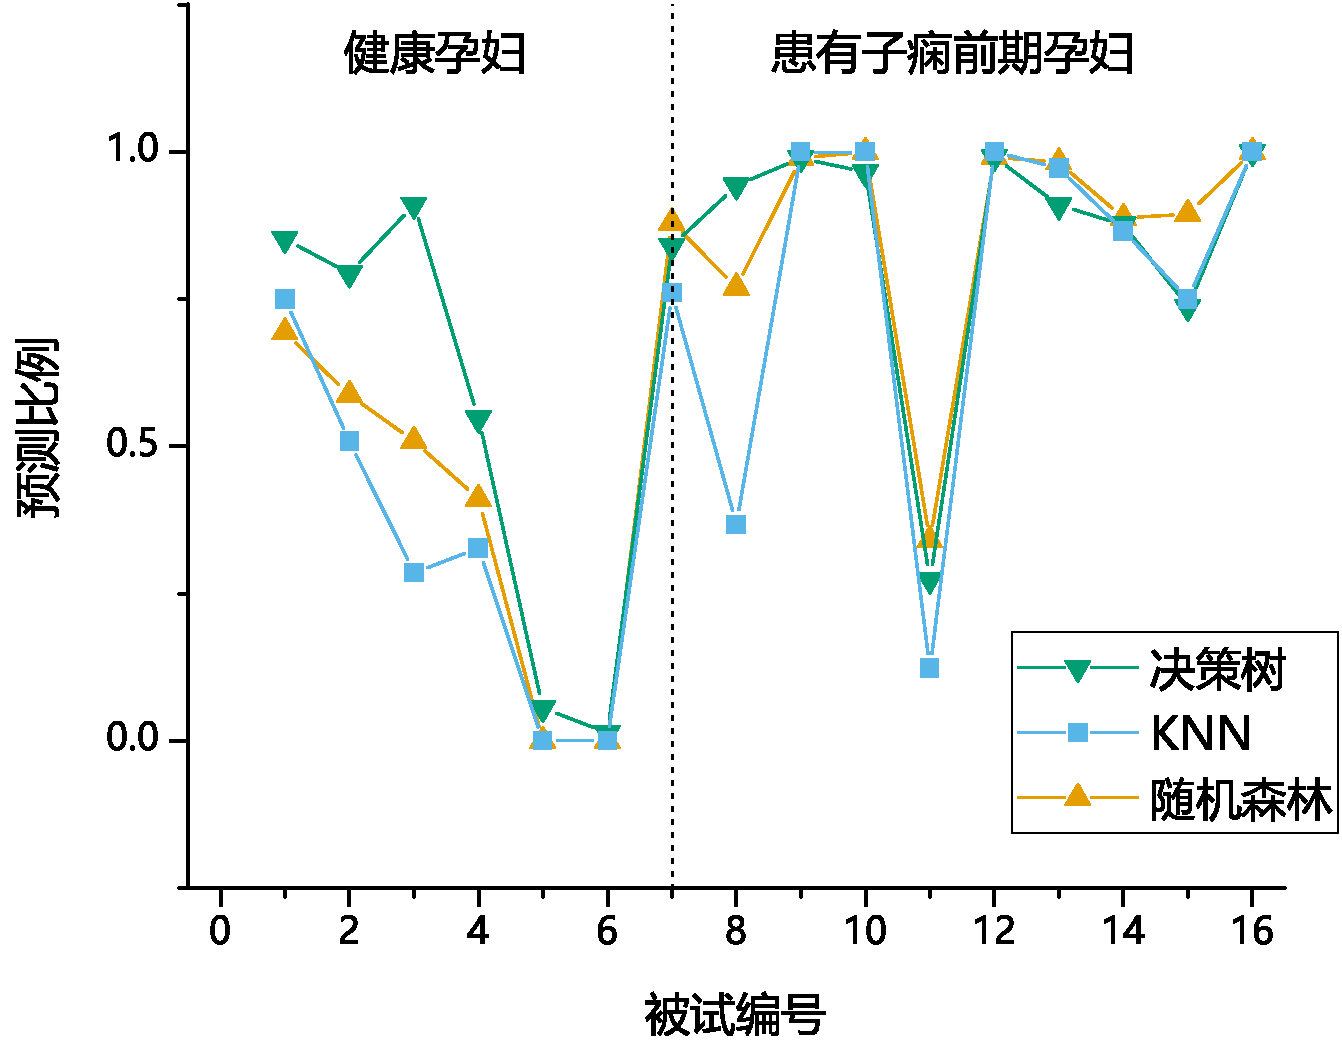
\includegraphics[width=7.5cm]{results/detail_31}
      }
      \quad
      \subfigure[\label{fig:detail_32}对脉搏波进行重采样处理得到的预测比例散点图]{
      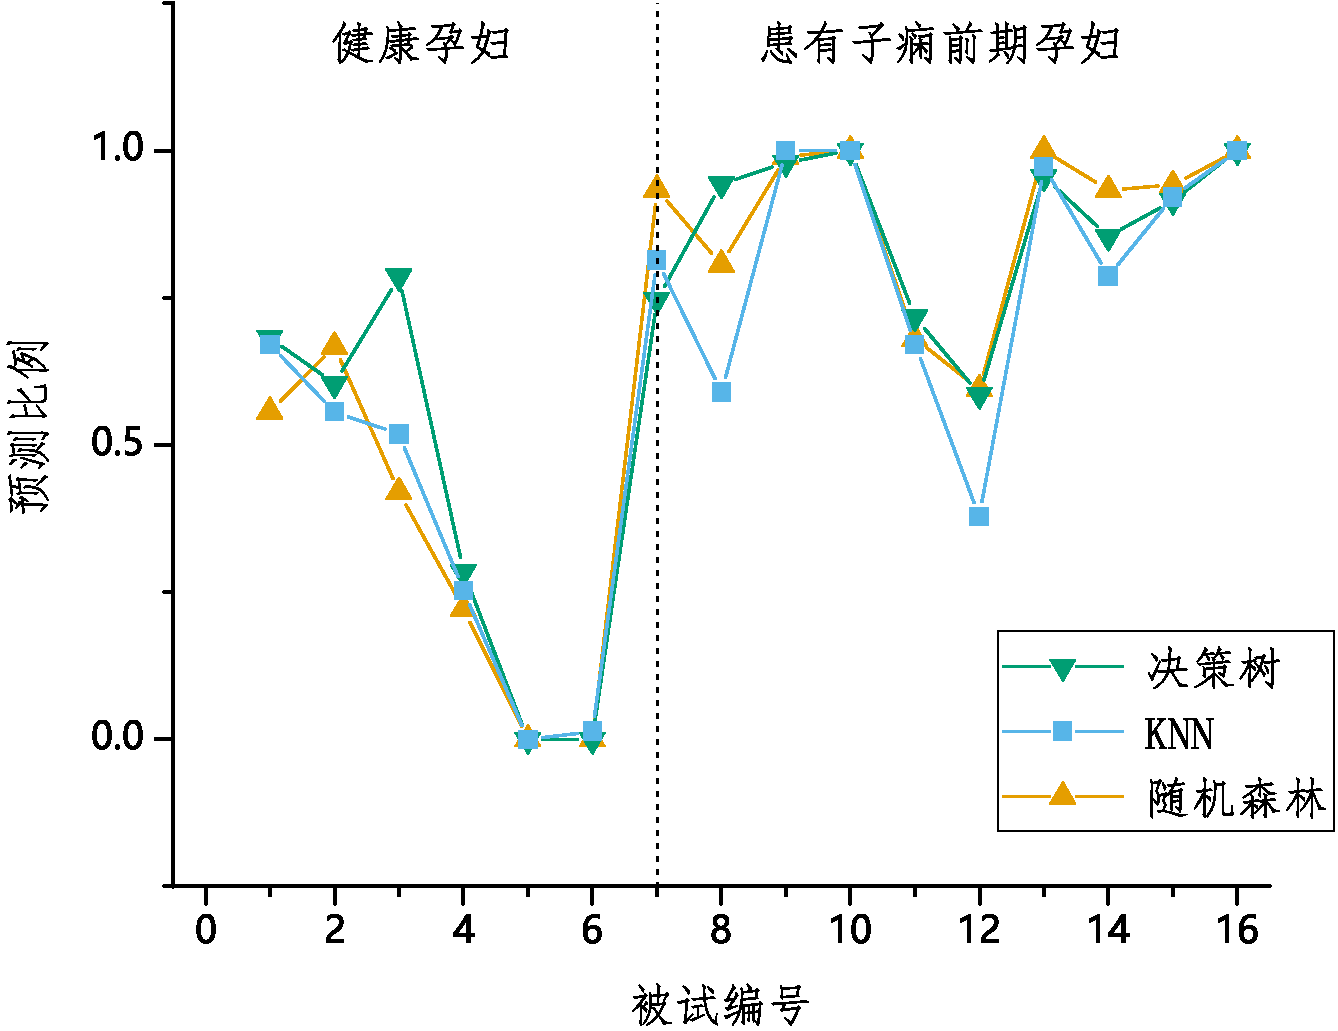
\includegraphics[width=7.5cm]{results/detail_32}
      }
      \caption{\label{fig:model_detail2}基于三种算法得到的子痫前期预测比例散点图2}
\end{figure}

在\autoref{tab:model_detail2}的基础上,将三种算法训练所得的模型在测试集上的预测比例作为该模型表征被试子痫前期患病状态的输出,则可以得到\autoref{fig:model_detail2}所示的散点图。此时,对子痫前期的识别分析可以转换为寻找
能将\autoref{fig:model_detail2}进行最佳分割的阈值。遍历各模型的预测比例数值并将该数值作为分割阈值,可以得到在该数值下的混淆矩阵,并进一步得到该数值对应的敏感性与特异性。最终,三种模型的预测比例
所对应的ROC曲线如\autoref{fig:model_roc2}所示。其中,将脉搏波进行补零处理后,决策树、K近邻及随机森林三种模型对应的AUC数值分别为0.825、0.849及0.905;将脉搏波进行重采样处理后,三种模型对应的AUC数值分别为0.905、0.865及0.929。
同时,将脉搏波进行补零处理后,借助约登指数可以确定三种模型的最佳分割阈值分别为0.864、0.813与0.884;将脉搏波进行重采样处理后,最佳阈值分别为0.573、0.820与0.673。各模型在最佳阈值下的
混淆矩阵如\autoref{tab:cm_on_best2}所示。将脉搏波进行补零处理后,三种模型的整体识别准确率分别为81.3\%、81.3\%与81.3\%;而将脉搏波重采样后,三种模型的整体识别准确率分别为87.5\%、81.3\%与87.5\%。

\begin{figure}[htbp]
      \centering
      \subfigure[\label{fig:roc_31}按脉搏波进行补零处理得到的预测比例得到的ROC曲线]{
      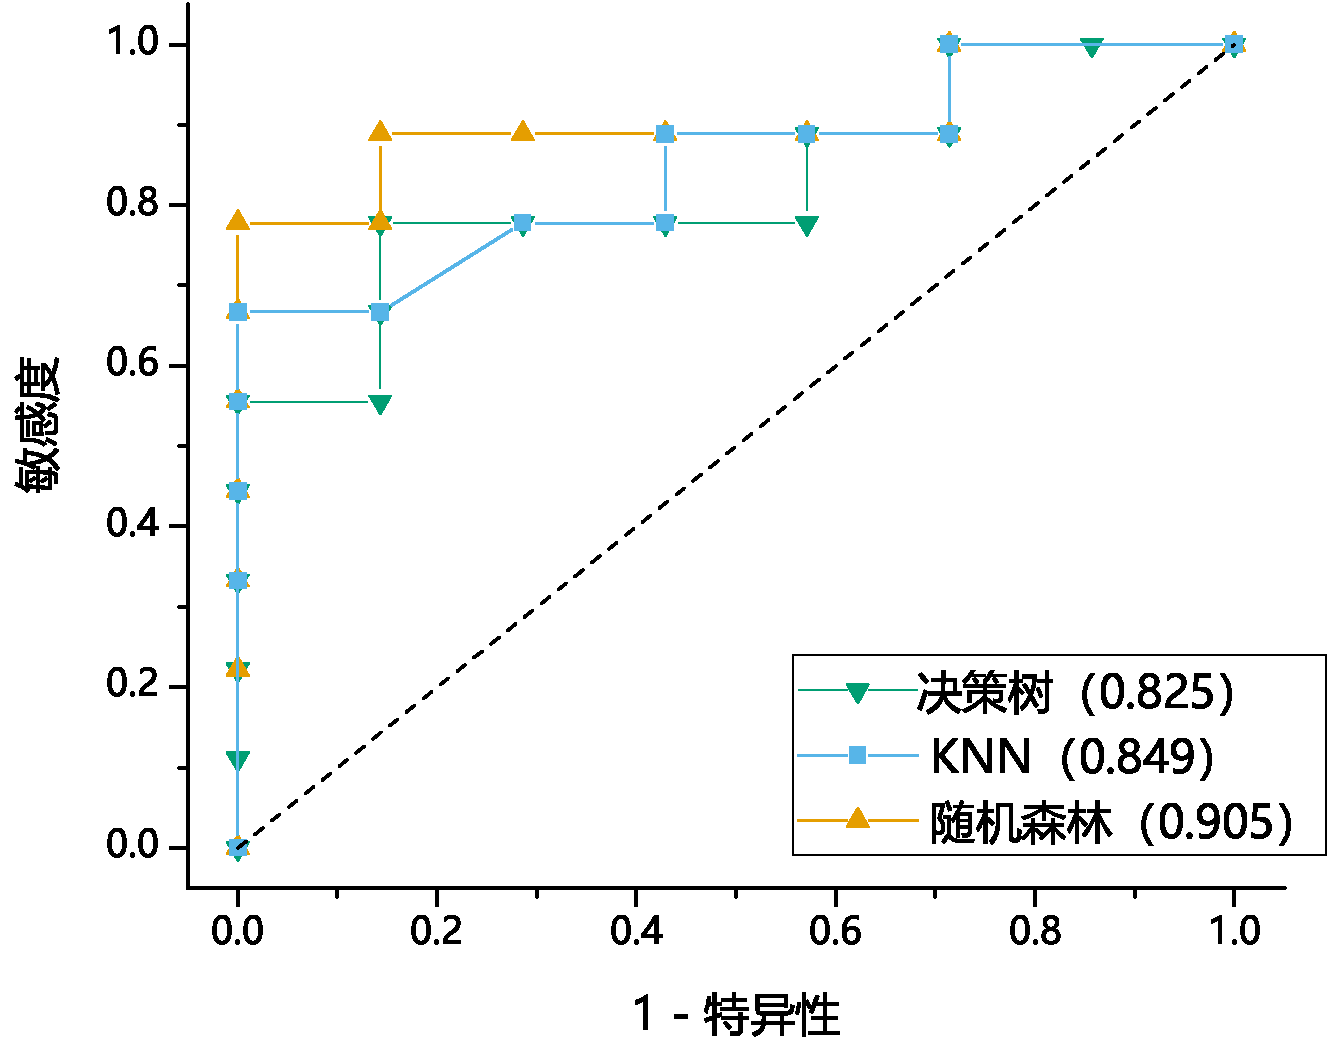
\includegraphics[width=7.5cm]{results/roc_31}
      }
      \quad
      \subfigure[\label{fig:roc_32}按脉搏波进行重采样处理得到的预测比例得到的ROC曲线]{
      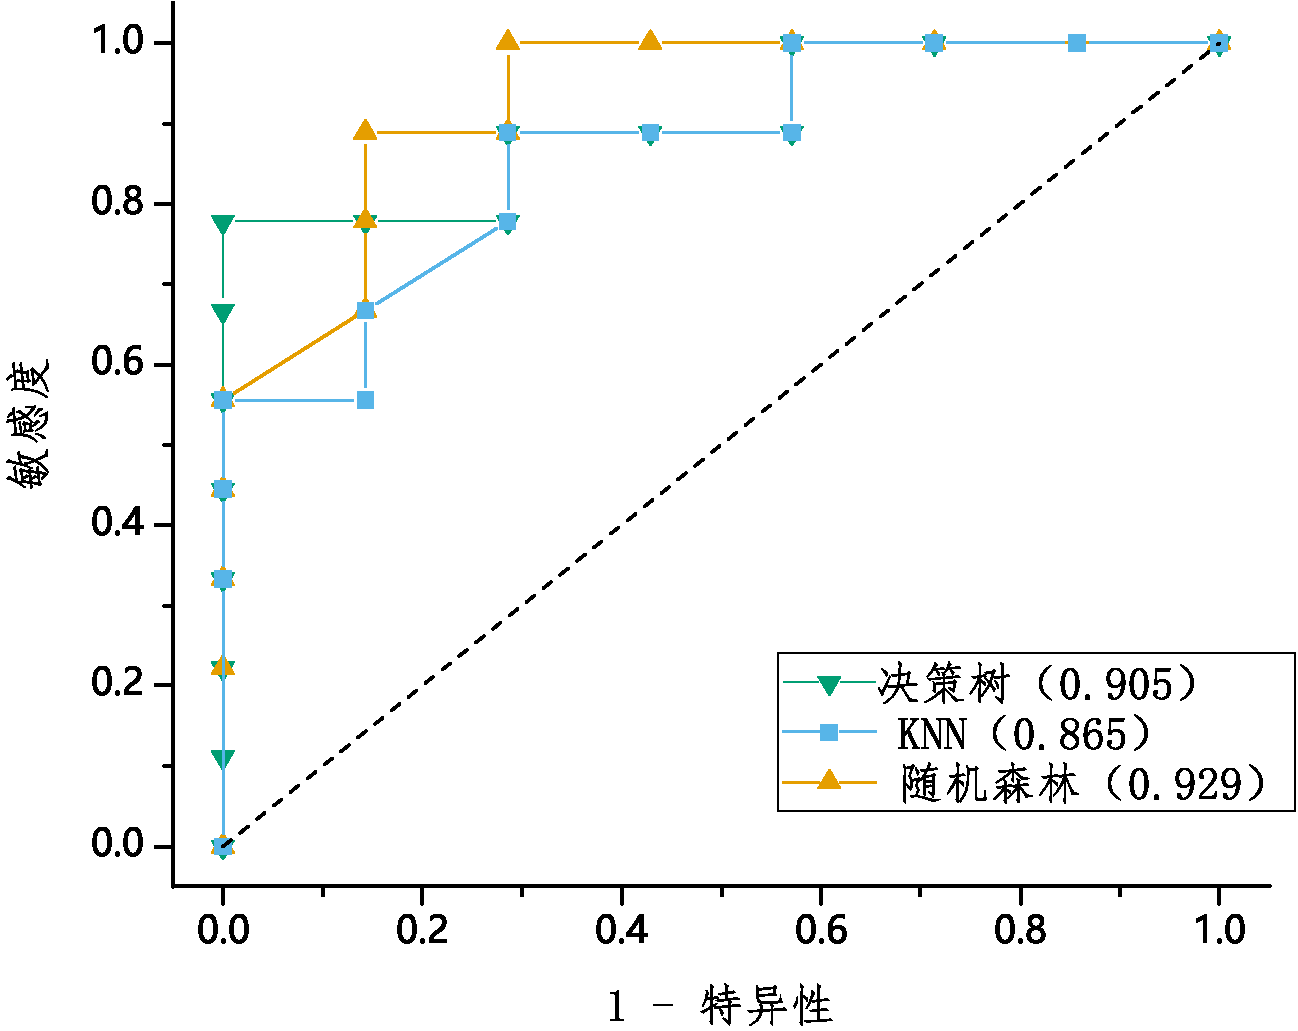
\includegraphics[width=7.5cm]{results/roc_32}
      }
      \caption{\label{fig:model_roc2}由子痫前期预测比例得到的 ROC 曲线2}
\end{figure}

\begin{table}[htbp]
      \zihao{5}
      \centering
      \caption{\label{tab:cm_on_best2}三种模型在最佳分割阈值下的混淆矩阵}
      \begin{tabular}{cccc}
      \toprule
      \textbf{脉搏波对齐方式}&\textbf{决策树算法}&\textbf{K近邻算法}&\textbf{随机森林算法}\\
      \midrule
      补零&$\left[ \begin{array}{cc} 7 & 2 \\ 1 & 6 \end{array} \right]$ & $\left[ \begin{array}{cc} 6 & 3 \\ 0 & 7 \end{array} \right]$ & $\left[ \begin{array}{cc} 7 & 2 \\ 1 & 6 \end{array} \right]$ \\
      重采样&$\left[ \begin{array}{cc} 7 & 2 \\ 0 & 7 \end{array} \right]$ & $\left[ \begin{array}{cc} 8 & 1 \\ 2 & 5 \end{array} \right]$ & $\left[ \begin{array}{cc} 8 & 1 \\ 1 & 6 \end{array} \right]$ \\
      \bottomrule
      \end{tabular}%
\end{table}%

从上述研究结果中可以得到以下结论:

1、在按被试划分原始数据集后,再进行子痫前期识别模型的训练,所得的子痫前期预测比例具有一定的子痫前期识别能力。借助AUC与ROC分析,在两种脉搏波对齐处理方式下,三种算法均可达到81.3\%以上的整体准确率。

2、从\autoref{fig:model_roc2}来看,在K近邻、决策树及随机森林等三种分类算法构建的识别模型中,随机森林模型有着最佳的分类效果,在两种脉搏波对齐处理方式下均能取得其最大的AUC数值(0.905与0.929),
而K近邻算法与决策树算法则各有优劣。

3、从\autoref{tab:cm_on_best2}来看,K近邻算法识别的总体准确率在两种脉搏波对齐处理方式下均为最低,而决策树与随机森林的整体性能极为接近。

4、从最佳分割阈值来看,将脉搏波补零处理时,三种算法的分割阈值较大,有泛化能力不足的潜在风险;而将脉搏波重采样后,决策树与随机森林模型的分割阈值则相对适中(0.573与0.673)。

\section{综合讨论与分析}
本小节在回顾前两节中的研究内容的基础上,进一步对以下问题进行讨论与分析。

一、数据集划分方式

第四章已经介绍过,在将新型时域波形描述特征集及脉搏波原始采样点按照全部波形与被试进行分层抽样、划分训练集与测试集的根本目的是为了弥补
本研究采集使用的实验数据较少。本章则在这两种数据集划分方式的基础上,分别进行了子痫前期识别模型的建立与研究。
结果表明\textbf{通过本研究提出的新型时域波形描述特征集及脉搏波原始采样点均能构建出具体一定子痫前期识别能力的机器学习模型,也即说明新型时域波形描述特征集及脉搏波原始采样点中
包含了能够表征子痫前期与正常妊娠孕妇形态差异的特征}。

\textbf{按照全部波形进行子痫前期识别模型的研究过程,实际上基于子痫前期导致的病生理变化可以在单个波形上得到体现的假设。}在这种假设中,单个脉搏波波形也包含了
识别子痫前期的全部信息。\textbf{按照被试人群进行子痫前期识别模型的研究过程,实际上基于子痫前期导致的病生理变化是通过被试全部脉搏波的多数波形的形态特征来反应的假设。}
在该假设中,同一被试的全部脉搏波波形的形态整体“群体决策”了该被试的子痫前期状态。

另一方面,在按全部波形进行训练集与测试集的划分时,同一被试的不同脉搏波波形可能会分别被划分至训练集与测试集。若这些波形高度相似,就可能最终的模型识别准确率较高。
因此,有必要按被试划分训练集与测试集的划分,确保同一被试的波形数据只出现在训练集或测试集。由于测试集对最终生成的模型而言是全新的数据,这种方式下对模型的泛化能力的评估更为有效。

最后从数值结果来看,本章的研究结果为上述两种猜想均提供了一定支撑。基于本研究提出的新型时域波形描述特征集及脉搏波原始采样点,按照两种数据集的划分方式,使用
多种机器学习训练得到的模型均有一定的子痫前期识别能力。

二、机器学习模型的影响

本研究在经过多种机器学习算法的初筛后,着重考察了两种单模型算法决策树与K近邻算法——与一种集成算法——随机森林——构建子痫前期识别模型的效果。
通过上述算法在本研究涉及了多种场景下的分析生成的子痫前期识别模型在测试集上性能表现(仅以准确率为例进行统计)如\autoref{tab:accuracy}所示。

\begin{table}[htbp]
      \zihao{-5}
      \centering
      \caption{\label{tab:accuracy}不同分析场景下通过三种算法模型在测试集上准确率对比}
      \begin{tabular}{cccccc}
      \toprule
      \textbf{数据集}&\textbf{抽样方式}&\textbf{随机森林}&\textbf{K近邻}&\textbf{决策树}&\textbf{备注}\\
      \midrule
      \multirow{3}{*}{新型时域波形描述特征集} & 全部波形 & 97.0\% & 93.3\% &  88.9\%& \\
            & 被试 & 79.1\% & 78.3\% & 66.3\% & 按波形统计\\
            & 被试 & 93.8\% & 81.3\% & 81.3\% & 计算预测比例后按被试统计\\
      \multirow{6}{*}{脉搏波采样点} & 全部波形 & 93.6\% & 91.4\% & 86.2\% & 脉搏波补零对齐\\
                  & 全部波形 & 92.5\% & 91.6\% & 83.9\% & 脉搏波重采样对齐\\
                  & 被试 & 74.3\% & 78.3\% & 67.5\% & 脉搏波补零对齐,按波形统计\\
                  & 被试& 77.0\% & 74.7\% & 71.6\% & 脉搏波重采样对齐,按波形统计\\
                  & 被试 & 81.3\% & 81.3\% & 81.3\% & 脉搏波补零对齐,计算预测比例后按被试统计\\
                  & 被试& 87.5\% & 81.3\% & 87.5\% & 脉搏波重采样对齐,计算预测比例后按被试统计\\      
      \bottomrule
      \end{tabular}%
\end{table}%

从\autoref{tab:accuracy}可以发现,\textbf{随机森林算法充分体现了集成学习的优势,在本研究涉及的多种分析场景下,随机森林算法构建的模型性能均高于决策树算法与K近邻算法。
而对于决策树与K近邻算法,在大多数分析场景下,K近邻算法的性能表现优于决策树算法。}

三、特征集的影响

进一步考察\autoref{tab:accuracy}中使用的数据集对最终子痫前期识别模型在测试集上准确率可以发现,\textbf{本研究提出的新型时域波形描述特征集及脉搏波原始采样点在子痫前期的识别能力上具有一致性。}
在相同的研究场景中,使用相同算法在两类时域特征集构建的模型在测试集上的准确率数值极为接近,且均是在新型时域波形描述特征集上的构建模型性能优于在脉搏波原始采样点上构建的模型。
这也表明,\textbf{相较而言,新型时域波形描述特征集表征子痫前期的能力要强于脉搏波原始采样点。这也说明本研究提出的新型时域波形描述特征集设计合理,有应用于与本研究类似的基于脉搏波的其他相关研究的潜力}。

四、特征贡献与分布

本研究在新型时域波形描述特征集及脉搏波原始采样点上均按全部波形进行抽样后构建了子痫前期识别模型。特别地,当使用随机森林算法构建模型时,可以评估参与模型构建的特征的贡献度。
对比\autoref{tab:rf_dr_1}与\autoref{fig:rf_imp2},关于
新型时域波形描述特征集及脉搏波原始采样点在贡献度可以得到以下结论:

1、新型时域波形描述特征集与脉搏波原始采样点贡献度的最大值有一定差异,前者的最大值可以到达整体平均值的13.6倍以上,而后者仅为均值的6倍左右。这说明新型时域波形描述特征集中,与子痫前期相关
的特征更为明显。

2、对比两种脉搏波时域特征集上得到各特征的贡献度分布可以发现,两类时域特征集中具有子痫前期表征能力的特征出现的位置高度相似。贡献度高的特征多出现在下降支中,且集中在下降支的前端与尾端。这点在
\autoref{fig:rf_imp2}体现得更为明显,在特征贡献度分布中,脉搏波峰值之后及尾端位置出现了两个分布高峰。\textbf{这种现象也与脉搏波
下降支是血液回流过程的反应、下降支包含了更多的血液循环中细节信息的、子痫前期
会影响孕妇血液循环等事实相符合。说明这些位置的脉搏波形态可能是识别子痫前期的关键。}

\section{小结}
本小节通过新型时域波形描述特征集合与脉搏波原始采样点的基础上利用借助决策树、K近邻及随机森林等算法完成了不同分析场景下的子痫前期识别模型的构建与分析工作。
各模型在测试集上的性能表现证明生成的机器学习模型具有一定子痫前期识别能力的,也说明新型时域波形描述特征集及脉搏波原始采样点中
包含了能够表征子痫前期与正常妊娠孕妇形态差异的特征。而当横向对比三种机器学习算法的性能时,随机森林算法构建的子痫前期识别模型性能最好,K近邻次之,决策树最次。
而通过脉搏波新型时域波形描述特征集合构建的机器学习模型性能也要优于使用直接使用脉搏波原始采样点构建的模型。而从特征的角度而言,新型时域波形描述特征集合与脉搏波原始采样点中
具有子痫前期识别能力的特征出现的位置也高度相似,且与脉搏波的生理学基础有一定的对应关系。
